\subsection{Double-Moment Bulk \cite{sn_2014}}

\subsubsection{Treatment of hydrometeors}
Generally, characteristics of cloud particles are determined by their size, shape, and the chemical properties of solute within them. Representation of these characteristics requires a multi-dimensional parameter space of size, shape, and chemical compositions. Since development of a cloud resolving model (CRM) coupled with an aerosol transport model is beyond the scope of this study, we consider a two-dimensional parameter space of size and shape of cloud particles. We then categorize cloud models into two major groups, according to their representation of cloud particles. One is the bin method, using discretized particle size bins and predicting the population density of particles in each bin. The other is the bulk method, in which particle size distributions are approximated by several prescribed modes, predicting the total populations of particles of each mode. The treatment of hydrometeors adopted in this study is described in the following sections.

\subsubsection{Droplet Size Distribution}
The Seiki and Nakajima (2014)\cite{sn_2014} scheme is designed to maintain the self-consistency of assumptions regarding droplet size distribution (DSD) and the shapes of ice particles among cloud microphysical processes. Following Seifert and Beheng (2006; hereafter, SB06), Seiki and Nakajima(2014)\cite{sn_2014} predict the moments of the DSD of each hydrometeor, assuming generalized gamma distribution to analytically formulate cloud microphysics, as follows:

\begin{eqnarray}
f_{a}(r)=\alpha_{a}x^{\nu_{a}}\exp(-\lambda x)
\label{sn7}
\end{eqnarray}

where the index a $\in$ (c,r,i,s,g) represents cloud water, rain, cloud ice, snow, and graupel. For a given DSD, the k-th moment can be defined as follows:

\begin{eqnarray}
M^{(k)}_{a}\equiv \int_{0}^{\infty}x^{k}f_{a}(r)dx,\;\;(k\in {\bf R})
\label{sn8}
\end{eqnarray}

For example, the 0-th moment of a DSD is the number concentration $N_{a}$, and the 1st moment is the mass concentration $L_{a} = \rho q_{a}$. The evolution of DSD is represented by updating $\alpha_{a}$ and $\lambda_{a}$ using $N_{a}$ and $L_{a}$ with two fixed parameters, $\nu_{a}$ and $\mu_{a}$, respectively. The diagnostic parameters $\alpha_{a}$ and $\lambda_{a}$ are calculated as follows:

\begin{eqnarray}
\alpha_{a}=\frac{\mu_{a}\lambda_{a}}{\Gamma\Bigl(\frac{\nu_{a}+1}{\mu_{a}}\Bigr)}\lambda_{a}^{\frac{\nu_{a}+1}{\mu_{a}}}\\
\label{sn9}
\lambda_{a}=\Bigl[\frac{\Gamma\Bigl(\frac{\nu_{a}+1}{\mu_{a}}\Bigr)}{\Gamma\Bigl(\frac{\nu_{a}+2}{\mu_{a}}\Bigr)}\Bigr]^{-\nu_{a}}\nonumber
\end{eqnarray}

with mean particle mass $\bar{x}\equiv L_{a}/N_{a}$. We maintain the self-consistency of the shape of ice particles by assuming power law relationships between: 1) particle mass and maximum dimension D, and 2) particle mass and projected area to flow A, as follows:

\begin{eqnarray}
D&=&a_{m}x^{b_{m}}\\
\label{sn10}
A&=&a_{ax}x^{b_{m}}
\label{sn11}
\end{eqnarray}

where $a_{m}$, $b_{m}$, $a_{ax}$, and $b_{ax}$ are constant coefficients. We chose to use constant parameters for DSD representation, following SB06 for cloud water, cloud ice, snow, and graupel, and following Seifert (2008) for rain (assuming collisional-breakup equilibrium conditions). The shapes of ice particles are those given by Mitchell (1996), assuming cloud ice as hexagonal plates, snow as assemblages of planar polycrystals in cirrus clouds, and graupel as lump graupel. The above-mentioned constant parameters for each hydrometeor are summarized in Table \ref{table_sn14-1}.

\begin{table}[h]
\begin{center}
\caption{Constant parameters chosen for the generalized gamma distribution; power law coefficients used for maximum dimensions and projected area, and ranges of lower- and upper limits of mean mass.}
\label{table_sn14-1}
\scalebox{0.85}{
\begin{tabular}{cccccc}
\hline
                         & cloud water   & rain    & cloud ice   & snow   & graupel   \\ \hline\hline
$\nu$                    & 1  & -1/3 & 1 & 1 & 1 \\ \hline
$\mu$                    & 1  &  1/3 & 1/3   & 1/3   & 1/3   \\ \hline
$a_{m}$[m $kg^{-bm}$]    & 0.124   & 0.124   & 1.24   & 1.24   & 0.346   \\ \hline
$b_{m}$                  & 1/3 & 1/3 & 0.408   & 0.408   & 0.357 \\ \hline
$a_{ax}$[$m^{2}$$kg^{-bA}$]    & 0.0121   & 0.0121   & 0.178   & 0.196   & 0.0599   \\ \hline
$b_{ax}$ & 2/3 & 2/3 & 0.755   & 0.768   & 0.714 \\ \hline
$\bar{x_{min}}[kg]$ & $4.2\times 10^{-12}$ & $4.2\times 10^{-12}$ & $4.2\times 10^{-12}$ & $4.2\times 10^{-12}$ & $4.2\times 10^{-12}$ \\ \hline
$\bar{x_{max}}[kg]$ & $2.6\times 10^{-10}$ & $2.6\times 10^{-10}$ & $2.6\times 10^{-10}$ & $2.6\times 10^{-10}$ & $2.6\times 10^{-10}$ \\ \hline
\end{tabular}
}
\end{center}
\end{table}

\subsubsection{Terminal velocity of hydrometeors}
In the same manner as Seifert and Beheng (2006a), the terminal velocities of particles are formulated in power laws, except for gravitational sedimentation, which is described using an accurate formula because it is directly compared with precipitation data. The terminal velocities of hydrometeors are determined by the balance between drag and gravitational forces. Traditionally, the terminal velocities for small spherical particles with small Reynolds number ($N_{Re}$) are described by Stokes’ Law:

\begin{eqnarray}
\nu_{t,stokes}(r)=\frac{2g(\rho_{w}-\rho)}{9\eta_{a}}r^{2}
\label{sn12}
\end{eqnarray}

where $g$ = 9.80616 $[m s^{-2}]$ is gravitational acceleration, $\rho w$ = 1000 $kg m^{-3}$ is the density of liquid water, $\rho$ is the density of air, and $\eta_{a}$ is the dynamic viscosity of air. Laboratory experiments have shown that terminal velocity departs from Stokes’ Law as the Reynolds number increases (Gunn and Kinzer, 1948; Beard and Pruppacher, 1969). Other formulas are thus required for larger droplets, such as rain droplets and ice crystals.\\
In the case of liquid water droplets, terminal velocity can be determined well by laboratory experiments because of the simplicity of shape. In contrast, there are many observed terminal velocities of ice particles for various shapes of ice crystals. Bohm (1989), Bohm (1992), and Mitchell (1996) proposed general formulations of the terminal velocities of ice particles based on the boundary layer theory, with their studies showing good agreement with observational data. In this study, we calculated terminal velocities for each ice particle based on Mitchell (1996) and then created a fitting curve using a power law within a suitable diameter range. \\
In theoretical formulas, the terminal velocities of hydrometeors are dependent on diameter, shape, the Reynolds number, and the Best (or Davies) number ($N_{X}$). Applying these to cloud microphysics is extremely complicated; here, we therefore apply a simplified approach suggested by Beard (1980):\\
1. The terminal velocity is calculated for the reference atmosphere.\\
2. The terminal velocity in the atmosphere is adjusted from the reference value.\\
In the following paragraphs, we describe terminal velocities for the reference atmosphere and the adjustment technique.

\subsubsection{Terminal velocity of liquid water droplets for the reference atmosphere}
In the case of liquid water droplets, absence of shape variability makes formulation easier than in the case of ice particles. Here, we only consider dependency on the diameter of droplets. Seifert and Beheng (2006) applied the formulation of Rogers et al. (1993), the analytical approximation of Gunn and Kinzer’s (1948) observation data:

\begin{eqnarray}
\nu_{t}(D)=
\left\{
\begin{array}{l}
a_{R_{s}}D(1-exp(-b_{R_{s}}D)),\;\;(D<D_{0,r}) \\
a_{R_{l}}-b_{R_{l}}exp(-c_{R_{l}}D),\;\;(D>D_{0,r}) \\
\label{sn13}
\end{array}
\right.
\end{eqnarray}

where $a_{R_{s}}= 4000 s^{-1}$, $b_{R_{s}}=12000 m^{-1}$, $a_{R_{l}}=9.65 m s^{-1}$, $b_{R_{l}} = 10.43 m s^{-1}$, $c_{R_{l}} = 600 m^{-1}$, and $D_{0}$, $r=7.45\times10^{-4}$ m. This formulation approaches the quadratic form of Stokes’ Law in the limit for small diameters. In addition, Gunn and Kinzer’s (1948) data agrees well with the terminal velocities calculated via theoretical formulation based on the boundary layer theory (Bohm, 1992). We therefore applied eq.\ref{sn13} for rain sedimentation (Fig. \ref{figsn2-11}2 11). Here, the reference atmosphere of the formulation is $T = 293 K$, $p = 1000hPa$, and relative humidity is 0.5 (Gunn and Kinzer, 1948).

\subsubsection{Terminal velocity of solid water particles for the reference atmosphere}
In the case of ice particles, we derive the theoretical formulation of the terminal velocity based on Mitchell (1996). In general the aerodynamic drag force $F_{D}$ on a particle is expressed as follows:

\begin{eqnarray}
F_{D}\equiv \frac{1}{2}\rho\nu_{t}^{2}AC_{D}
\label{sn14}
\end{eqnarray}

where $C_{D}$ is the drag coefficient. Terminal velocity is determined by the equilibrium condition between the drag force and gravitational acceleration:

\begin{eqnarray}
\nu_{t}=\bigl(\frac{2xg}{\rho AC_{D}}\bigr)^{1/2}
\label{sn15}
\end{eqnarray}

The problem of derivation of the terminal velocity is reduced to derivation of the drag coefficient, independent of the terminal velocity. In practice, Mitchell (1996) and many other researchers calculated the terminal velocity by defining the Best number ($N_{X}$), as follows:

\begin{eqnarray}
N_{x}\equiv C_{D}N_{R_{e}}^{2}=\frac{2xg\rho D^{2}}{A\eta_{a}^{2}}
\label{sn16}
\end{eqnarray}

where $N_{R_{e}}$ is the Reynolds number. The terminal velocity can be calculated after the relationship between Best and Reynolds numbers is determined. In the relationship, it is convenient for the drag coefficient to be determined by the Reynolds number, although the dependency of the former is complicated. A theoretical formulation of the drag coefficient was proposed by Abraham (1970). The drag coefficient is the dimensionless number defined by the drag force, the dynamic pressure, and the projection area of the particle (see eq.\ref{sn14}). Abraham (1970) assumed that the effective projection area of the particle contained the projection area of the particle itself and also the boundary layer surrounding the particle, as follows:


\begin{eqnarray}
F_{D}=\frac{1}{2}\rho \nu_{t}^{2}C_{0}A\bigl(1+\frac{\delta_{b}}{r_{A}}\bigl)^{2}
\label{sn17}
\end{eqnarray}

where $C_{0}$ is the drag coefficient due to the pressure of the fluid and should be determined independently of the shape, $\delta_{b}$ is the boundary layer depth, and $r_{A}$ is the radius of a circle with the equivalent projection area. Furthermore, the ratio of boundary layer depth to radius is expressed as follows:

\begin{eqnarray}
\frac{\delta_{b}}{r_{A}}=\frac{\delta_{0}}{N_{R_{e}}^{1/2}}
\label{sn18}
\end{eqnarray}

where $\delta_{0}$ is a non-dimensional constant. Substituting eq.\ref{sn18} into eq.\ref{sn17}, the drag coefficient, which also includes the effect of the boundary layer, corresponds to the following:

\begin{eqnarray}
C_{D}=C_{0}\bigl(1+\frac{\delta_{0}}{N_{R_{e}}^{1/2}}\bigr)^{2}
\label{sn19}
\end{eqnarray}

The drag coefficient is thus expressed by the Reynolds number. The relationship between Reynolds and Best numbers is derived by substituting eq.\ref{sn19} into eq.\ref{sn16}:

\begin{eqnarray}
N_{R_{e}}=\frac{\delta_{0}^{2}}{4}\Bigl[\bigr(1+\frac{4N_{X}^{1/2}}{\delta_{0}^{2}C_{0}^{1/2}}\bigr)^{1/2}-1 \bigr]^{2}
\label{sn20}
\end{eqnarray}

Here we use $C_{0}$ = 0.6 and $\delta_{0}$ = 5.83, as provided by Bohm (1989). Finally the terminal velocity of ice particles is calculated by substituting eq.\ref{sn16} and eq.\ref{sn20} into the definition of the Reynolds number:

\begin{eqnarray}
\nu_{t}&=&\frac{N_{Re}\eta_{a}}{D\rho}\nonumber\\
&=&\frac{\eta_{a}}{D\rho}\frac{\delta_{0}^{2}}{4}\Bigl[\bigl[1+\frac{4}{\delta_{0}^{2}C_{0}^{1/2}}\bigr(\frac{2xg\rho D^{2}}{A\eta_{a}^{2}}\bigl)^{1/2}\bigr]^{1/2}-1\Bigr]^{2}
\label{sn21}
\end{eqnarray}

In this formulation, required variables are mass, projection area, maximum dimension of ice particles, and thermodynamical variables. Here we use several piecewise-constant mass-maximum dimension, and projection area-maximum dimension relationships provided by Mitchell (1996). The terminal velocities of various ice particles are plotted in Fig.\ref{figsn2-12}. As shown in Fig.\ref{figsn2-11}, there is less difference between hexagonal plates and stellar crystals with broad arms with diameter less than a few hundred micrometers. We therefore only consider hexagonal columns and hexagonal plates as representative of the ice category.


\subsubsection{Adjustment factor of terminal velocity}
Beard (1980) suggested that calculation of the terminal velocity using the Best number could be simplified with use of an adjustment factor ($f_{vt}$), defined as:

\begin{eqnarray}
\nu_{t}=\nu_{t0}f_{vt}
\label{sn23}
\end{eqnarray}

where $v_{t0}$ is a reference terminal velocity. He demonstrated that $f_{vt}$ was not sensitive to the shape of hydrometeors. When electrical force is not considered in cloud microphysics, formulas of $f_{vt}$ are as follows:

\begin{eqnarray}
f_{vt}&=&f_{vt0}\;\;(N_{Re_{0}}\leq0.2)\label{sn24}\\
f_{vt}&=&f_{vt\infty}\;\;(N_{Re_{0}}\geq1000)\label{sn25}\\
f_{vt}&=&f_{vt0}\nonumber\\
&+&(f_{vt\infty}-f_{vt0})(1.61+lnN_{R_{e}0})/8.52\;\;(N_{Re_{0}}<1000)\label{sn26}\\
f_{vt0}&\equiv&(\eta_{0}/\eta)\label{sn27}\\
f_{vt\infty}&\equiv&(\rho_{0}/\rho)^{0.5}\label{sn28}\\
N_{R_{e}0}&\equiv&\rho_{0}Dv_{t0}/\eta_{0}\label{sn29}
\end{eqnarray}

The upper ( $N_{R_{e}}$ = 1000 ) and lower ( $N_{R_{e}}$ = 0.2 ) limits of the Reynolds number correspond to diameters of several millimeters and tens of micrometers, respectively. Seifert and Beheng (2006) applied a further simplified adjustment factor based on eqs.\ref{sn27} and \ref{sn28}, as follows:

\begin{eqnarray}
f_{vt,n}=(\rho_{0}/\rho)^{\gamma_{n}}, \;\;\;(n=c,r,i,s,g)
\label{sn30}
\end{eqnarray}

where $\gamma_{c}$ = 1.0 and $\gamma_{r}$ = $\gamma_{i}$ = $\gamma_{s}$ = $\gamma_{g}$ = 0.5 This simplified formula of the adjustment factor is intended to avoid dependency on the Reynolds number. However, $\gamma_{n}$ = 0.5 is only valid for high Reynolds number particles with diameters > several millimeters, as shown in eq.\ref{sn21}. The above formula therefore always underestimates the terminal velocity of cirrus clouds. Another simplified formula for cirrus clouds was suggested by Heymsfield and Iaquinta (2000), as follows:

\begin{eqnarray}
f_{vt}=(p/p_{0})^{-0.178}(T/T_{0})^{-0.394}
\label{sn31}
\end{eqnarray}

where $T_{0}$ = 233 K and $p_{0}$ = 300 hPa. By using these adjustment factors, we can only consider the terminal velocity for the reference atmosphere. Adjustment factors used for each hydrometeor in this study are summarized in Table \ref{table_sn14-2-8}:

\begin{table}[h]
\begin{center}
\caption{Adjustment factor for the reference terminal velocity.}
\label{table_sn14-2-8}
\scalebox{0.75}{
\begin{tabular}{cccccc}
\hline
           & cloud     & rain    & ice   & snow   & graupel   \\ \hline\hline
$f_{vt}$   & 1         & $(\rho_{0}/\rho)^{0.5}$ & $(p/p_{0})^{-0.178}(T/T_{0})^{-0.394}$ & $(p/p_{0})^{-0.178}(T/T_{0})^{-0.394}$ & $(p/p_{0})^{-0.178}(T/T_{0})^{-0.394}$ \\ \hline
\end{tabular}
}
\end{center}
\end{table}


\subsubsection{Weighted mean terminal velocity}
In gravitational sedimentation, mean terminal velocity weighted by the k-th moments of DSD (${\bf \bar{v_{k,nq}}}$) is calculated in a straightforward manner, as follows:

\begin{eqnarray}
\bar{v_{k,nq}}=\int_{0}^{\infty}x^{k}f_{nq}(x)v_{t,nq}(x)dx
\label{sn32}
\end{eqnarray}

However, the terminal velocity formulas, eqs.\ref{sn14} and \ref{sn21}, are too complicated to analytically integrate eq.\ref{sn32}. Seifert and Beheng (2006) and Seifert (2008) used the large branch of eq.\ref{sn14} for rain droplets and simple power laws derived by observation for other hydrometeors. Here, we provide more accurate formulations to calculate weighted terminal velocities.\\
As shown above, dependency of the terminal velocity on diameter varies across aerodynamical regimes. In other words, dependency varies with diameter range. We therefore first prepared two branches of the terminal velocities of hydrometeors (except for cloud droplets) so as to integrate DSDs analytically. For cloud droplets, we used the same power law provided by Seifert and Beheng (2006), based on Stokes’ law. For rain droplets, we directly used the formulation of eq.\ref{sn14}, which allows analytical integration of each branch. In contrast, we need to derive two fitting curves for ice particles. The formulation of the terminal velocity of ice particles is described as a power law of the diameter using the least-square method, as follows:

\begin{eqnarray}
v_{t,js}&=&a_{v,js}x^{b_{v,js}},\;\;(js=i,s,g)\label{sn33}\\
(RMSE)_{k,js}&=&\sum_{id=1}^{id_max}\bigl(ln\bar{v_{k,js,true}}(\bar{D_{id}})-ln\bar{v_{k,js}}(\bar{D_{id}})\bigr)^{2}\label{sn34}\\
\frac{\partial(RMSE)_{k,js}}{\partial a_{v,js}}&=&0,\:\frac{\partial (RMSE)_{k,js}}{\partial b_{v,js}}=0\nonumber\\
\bar{v_{k,js}}(\bar{D_{id}})&=&\int_{0}^{\infty}a_{v,js}x^{b_{v,js}+k}f(x,\bar{D_{id}},L)dx/L\nonumber\\
&=&a_{v,js}\frac{\Gamma\bigl(\frac{v_{js}+b_{v,js}+k+1}{\mu_{js}}\bigr)}{\Gamma\bigl(\frac{v_{js}+k+1}{\mu_{js}}\bigr)}
\Bigl[\frac{\Gamma\bigl(\frac{v_{js}+1}{\mu_{js}}\bigr)}{\Gamma\bigl(\frac{v_{js}+2}{\mu_{js}}\bigr)}\Bigr]^{b_{v,js}}\bar{x_{id,js}^{b_{v,js}}}\label{sn35}\\
\bar{v_{k,js,true}}(\bar{D_{id}})&=&\sum_{i=1}^{imax}x^{k}v_{t,js,true}f_{logD}(lnD_{i},\bar{D_{id}},L)\Delta ln D/L\nonumber
\end{eqnarray}

where $D_{1}=10\mu m$, $D_{imax}=10mm$, $i_{max}=1000$, and L is an arbitrary constant. The fitting ranges of the mean volume diameter in eq.\ref{sn34} are from 20 to 400 $\mu$m for the small branch and from 200 to 2000 $\mu m$ for the large branch. The derived parameters are summarized in Table \ref{table_sn14-2-9}.\\
Second, the terminal velocity with a certain mean diameter is calculated by interpolating between the two branches in the logarithmic scale of the diameter. We use the mean diameter weighted by the kth moments of DSD in the interpolation. The formulation of weighted terminal velocities of rain droplets and solid particles are as shown below:

\begin{eqnarray}
\bar{v_{k,nq}}&=&w_{k,nq}\bar{v_k,lrg,nq}+(1-w_{k,nq})\bar{v_{k,lrg,nq}},\;\;(nq=r,i,s,g)\label{sn36}\\
w_{k,r}&=&0.5(1+tanh(\pi ln(\bar{D_{k,r}}/D_{0,k,r})))\nonumber\\
w_{k,js}&=&max(0.0, \;min(1.0,0.5(1+ln(\bar{D_{k,js}}/D_{0,k,js}))))\;\;(js=i,s,g)\nonumber\\
\bar{D_{k,nq}}&=&\frac{\int_{0}^{\infty}D_{nq}(x)x^{k}f_{nq}(x)dx}{\int_{0}^{\infty}x^{k}f_{nq}(x)dx}\nonumber\\
              &=&\bar{D_{nq}}\frac{\Gamma\bigl(\frac{v_{nq}+b_{m,nq}+k+1}{\mu_{nq}}\bigr)}{\Gamma\bigl(\frac{v_{nq}+k+1}{\mu_{nq}}\bigr)}\Bigl[\frac{\Gamma\bigl(\frac{v_{nq}+1}{/mu_{nq}}\bigr)}{\Gamma\bigl(\frac{v_{nq}+2}{\mu_{nq}}\bigr)}\Bigr]^{b_{m,nq}}\label{sn37}\\
\bar{v_{k,sml,r}}&=&\frac{f_{vt,r}}{M_{r}^{k}}\int_{0}^{\infty}\bigl[a_{R_{s}}D(1-exp(-b_{R_{s}}D))\bigr]x^{k}N_{r}(D)dD\nonumber\\
&=&a_{R_{s}}\frac{(1+\mu_{D,r}+3k)}{\lambda_{D,r}}\nonumber\\
&\times&\Bigl[1-\bigl(1+\frac{b_{R_{s}}}{\lambda_{D,r}}\bigr)^{-2-\mu_{D,r}-3k}\Bigr]\bigl(\frac{\rho_{0}}{\rho}\bigr)^{1/2}\label{sn38}\\
\bar{v_{k,lrg,r}}&=&\frac{f_{vt,r}}{M_{r}^{k}}\int_{0}^{\infty}\bigl[a_{Rl}-b_{Rl}exp(-c_{Rl}D)\bigr]x^{k}N_{r}(D)dD\nonumber\\
&=&a_{Rl}-b_{Rl}\bigl(1+\frac{c_{Rl}}{\lambda_{D,r}}\bigr)^{-1-\mu_{D,r}-3k}\bigl(\frac{\rho_{0}}{\rho}\bigr)^{1/2}\label{sn39}\\
N_{r}(D)&=&N_{0,r}D^{-\mu_{D,r}}exp(-\lambda_{D,r}D)
\end{eqnarray}

where $D_{0,r}$ and $D_{0,js}$ are the branch points of the fitting curves (see Table \ref{table_sn14-2-10}). Here we apply the form of the modified gamma distribution for diameter as a DSD of rain droplets. Derivation and correspondences of the coefficient $N_{0,r}$, the slope parameter $\lambda_{D}$,$r$, and shape parameter $\mu D$ appearing in the modified gamma distribution are described in Appendix B. Weighted terminal velocities of ice particles for two branches are calculated by eq.\ref{sn35}. Fig.\ref{figsn2-13} shows the terminal velocity of rain droplets weighted by number and mass concentration. Our method gives better results than those obtained using the approximated method adopted by Seifert and Beheng (2006) in the range within their upper and lower limits. Fig.\ref{figsn2-14} shows terminal velocities of ice particles weighted by number and mass concentration.


\begin{table}[h]
\begin{center}
\caption{Coefficients and exponents of the relationship between mass and terminal velocity of each hydrometeor used in gravitational sedimentation and other processes.}
\label{table_sn14-2-9}
\scalebox{0.5}{
\begin{tabular}{cccccc}
\hline
Hydrometeors & Sedimentation of mass & Sedimentation of mass & Sedimentation of number   & Sedimentation number & other process   \\ \hline\hline
             & Small                 & Large                 & Small                     & Large                 &                 \\ \hline
Cloud        & $a_{v}=3.75\times10^{5},b_{v}=2/3$ & $a_{v}=3.75\times10^{5},b_{v}=2/3$ & $a_{v}=3.75\times10^{5},b_{v}=2/3$ & $a_{v}=3.75\times10^{5},b_{v}=2/3$ & $a_{v}=3.75\times10^{5},b_{v}=2/3$ \\  \hline
Rain         & \ref{sn14}            & \ref{sn14}            & \ref{sn14}                & \ref{sn14}           & \ref{sn14}      \\ \hline
Hexagonal plate & $a_{v}=5800,b_{v}=0.505$ & $a_{v}=167,b_{v}=0.325$ & $a_{v}=1.24\times10^{5},b_{v}0.549$ & $a_{v}=422,b_{v}=0.385$ & $a_{v}=5800,b_{v}=0.505$\\ \hline
Hexagonal columns & $a_{v}=2900,b_{v}=0.466$ & $a_{v}=32.2,b_{v}=0.224$ & $a_{v}=9698,b_{v}0.531$ & $a_{v}=64.2,b_{v}=0.274$ & $a_{v}=2900,b_{v}=0.466$\\ \hline
Aggregates of planar polycrystals & $a_{v}=1.52\times10^{5},b_{v}=0.528$ & $a_{v}=306.0,b_{v}=0.330$ & $a_{v}=2.93\times10^{5},b_{v}0.567$ & $a_{v}=818,b_{v}=0.394$ & $a_{v}=1.52\times10^{5}b_{v}=0.528$\\ \hline
Lump graupel & $a_{v}=1.55\times10^{5},b_{v}=0.535$ & $a_{v}=312.0,b_{v}=0.330$ & $a_{v}=2.76\times10^{5},b_{v}0.571$ & $a_{v}=698,b_{v}=0.387$ & $a_{v}=1.55\times10^{5}b_{v}=0.535$\\ \hline
\end{tabular}
}
\end{center}
\end{table}

\begin{table}[h]
\begin{center}
\caption{Branch points of the weighted terminal velocity.}
\label{table_sn14-2-10}
\scalebox{0.75}{
\begin{tabular}{cc}
\hline
Hydrometeors & branch points of weighted terminal velocity [m] 
\\ \hline
Cloud        & Not used \\ \hline
Rain         & $D_{0,r}=7.45\times10^{-4}$ \\ \hline
Hexagonal plates & $D_{0,0,i}=262\times10^{-6}, D_{0,1,i}=399\times10^{-6}$ \\ \hline
Hexagonal columns& $D_{0,0,i}=240.5\times10^{-6}, D_{0,1,i}=330\times10^{-6}$ \\ \hline
Aggregates of planar polycrystals & $D_{0,0,s}=270\times10^{-6}, D_{0,1,s}=270\times10^{-6}$ \\ \hline
Lump graupel & $D_{0,0,g}=269\times10^{-6}, D_{0,1,g}=376\times10^{-6}$ \\ \hline
\end{tabular}
}
\end{center}
\end{table}

\begin{figure}[htbp]
\begin{center}
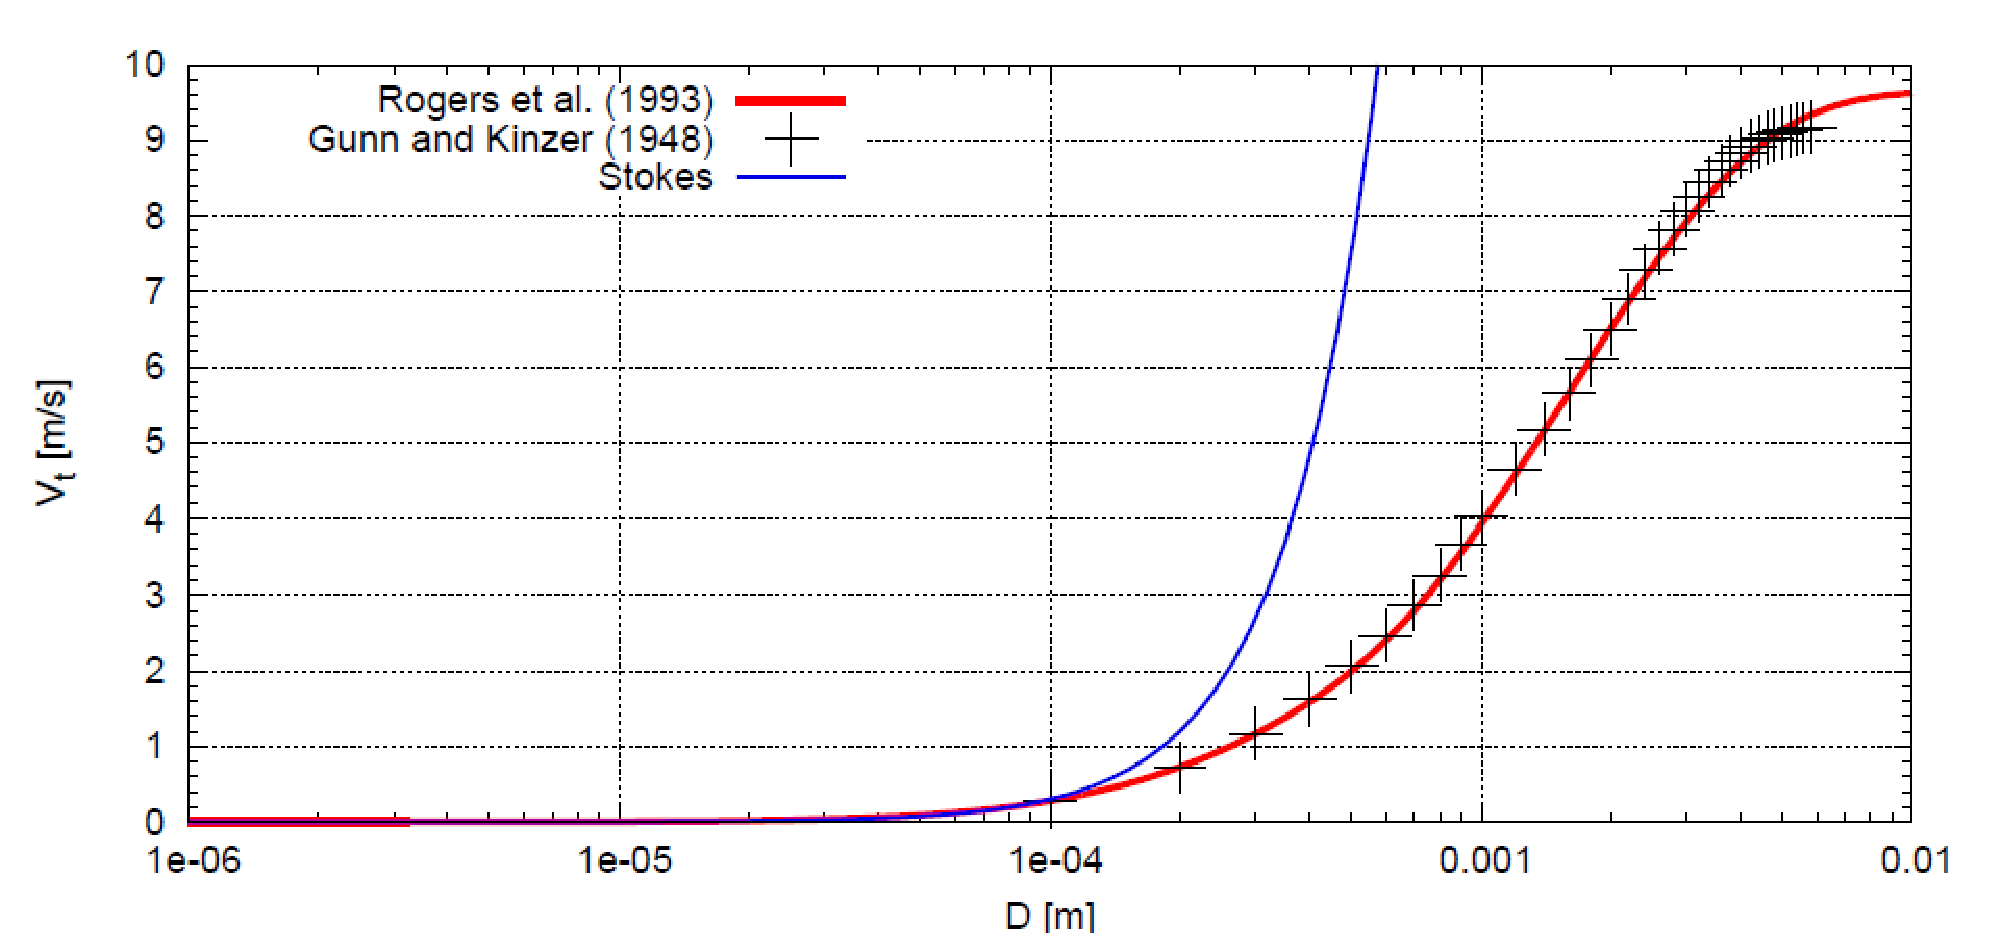
\includegraphics[scale=0.3]{./figure/D_vt_sn14.eps}
\end{center}
\caption{Dependency of terminal velocity of liquid water droplet on diameter. Marks are from Gunn and Kinzer (1948), red line is from Rogers et al. (1993), and blue line is calculated by Stokes’ law (eq.\ref{sn12}) under the condition T=293K, p=1000hPa.}
\label{figsn2-11}
\end{figure}

\begin{figure}[htbp]
\begin{center}
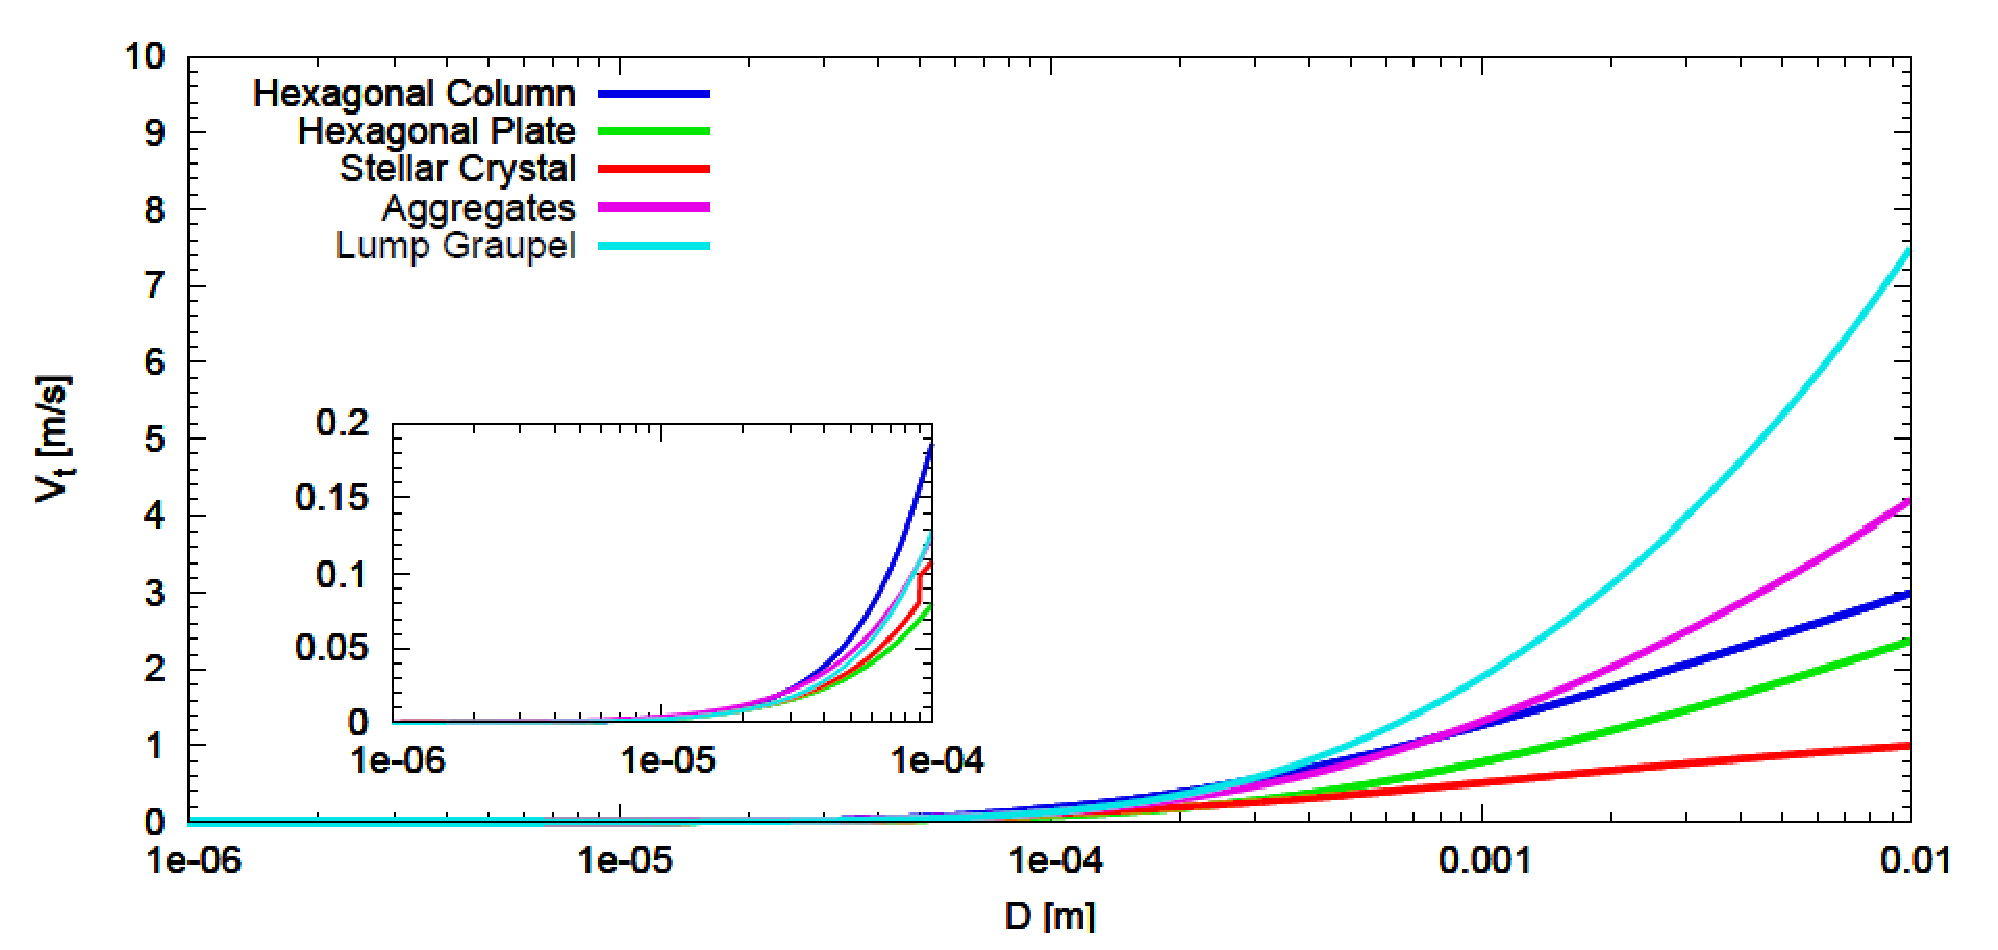
\includegraphics[scale=0.3]{./figure/D_vt_sn14-ice.eps}
\end{center}
\caption{Dependency of terminal velocity of liquid water droplet in maximum dimension. Each solid line color corresponds to different ice particle types, based on Mitchell (1996). Hexagonal columns are blue, hexagonal plates are green, stellar crystals with broad arms are red, aggregates of planar polycrystals in cirrus clouds are purple, and lump graupel is light blue.}
\label{figsn2-12}
\end{figure}

\begin{figure}[htbp]
\begin{center}
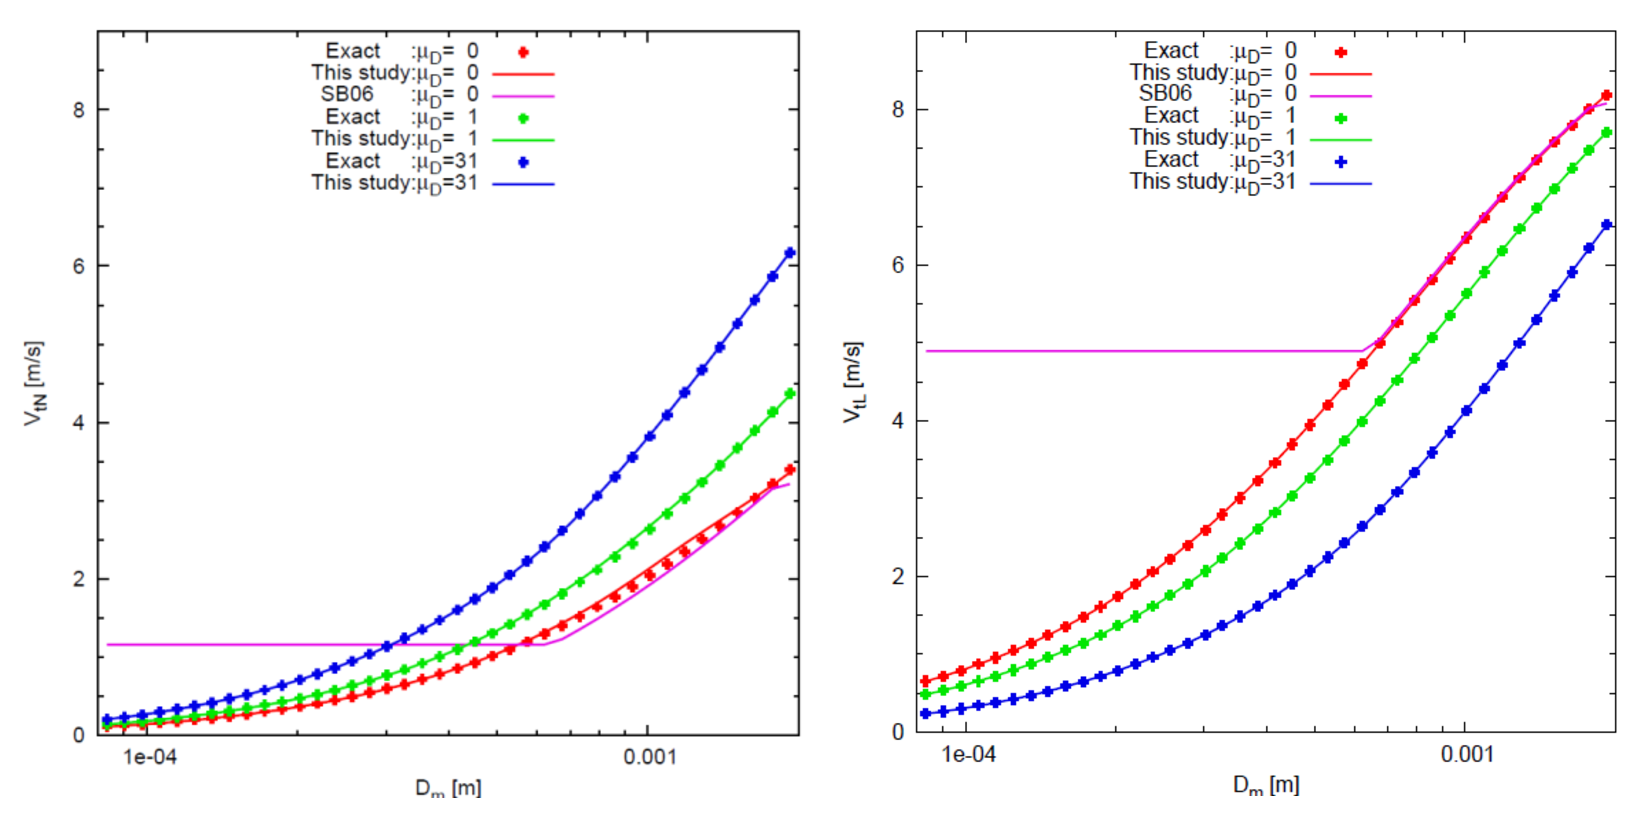
\includegraphics[scale=0.4]{./figure/D_vt_sn14-1.eps}
\end{center}
\caption{Dependencies of number weighted terminal velocity ($v_{tN}$) (left) and mass weighted terminal velocity ($v_{tL}$) (right) of rain droplets on mean volume diameter ($D_{m}$). Abscissa is the mean volume diameter and vertical axis is the terminal velocity. Dots show exactly integrated values and solid lines show approximated values obtained in this study (red, green, and blue) and by Seifert and Beheng (2006) (purple). Red and purple lines are calculated with $\mu D$ = 0, green lines are calculated with $\mu D$ = 1, and blue lines are calculated with $\mu D$ = 31.}
\label{figsn2-13}
\end{figure}

\begin{figure}[htbp]
\begin{center}
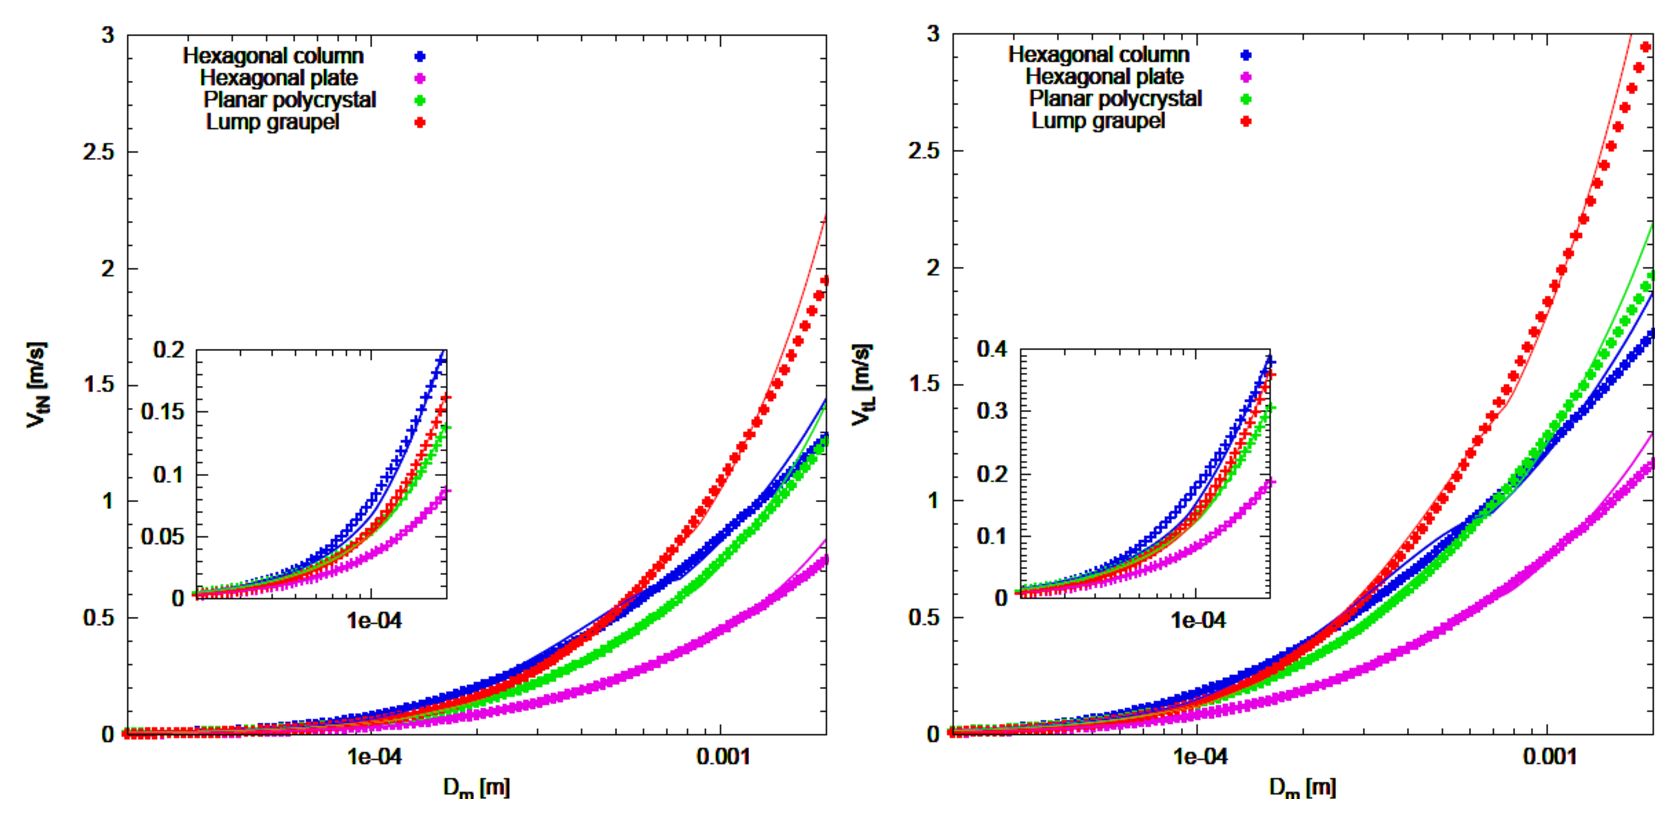
\includegraphics[scale=0.4]{./figure/D_vt_sn14-ice-1.eps}
\end{center}
\caption{Dependencies of number weighted terminal velocity ($v_{tN}$) (left) and mass weighted terminal velocity ($v_{tL}$) (right) of ice particles on mean volume diameter ($D_{m}$). Abscissa is the mean volume diameter and vertical axis is the terminal velocity. Dots show the exact value calculated by Mitchell (1996) and solid lines show the fitting curves. Red, green, blue, and purple denote lump graupels, assemblages of planar polycrystals, hexagonal columns, and hexagonal plates, respectively.}
\label{figsn2-14}
\end{figure}

\subsubsection{Detailed description of cloud microphysics}
Cloud microphysics is mainly subdivided into two. One is phase change among gas, liquid, and solid phases, while the other is the collection process among all particles. In addition, all hydrometeors are vertically transported by gravitational sedimentation. Phase change depends on the thermodynamics of environment air and itself affects thermodynamics through latent heat release. In contrast, collection is an internal growth process with less interaction with the atmosphere. Since the growth speed of the collection process is much faster than that of phase change, the role of the collection process is key to determining the lifetime of clouds (e.g., lifetime effect). Finally, gravitational sedimentation determines the removal rate of clouds from the atmosphere. It removes cloud directly by transportation, and indirectly by the collection process via collision volume (swept volume).\\
The cloud microphysics scheme developed in this study basically follows Seifert and Beheng (2006). Their two-moment bulk cloud microphysics scheme is remarkable in improvement of the collection process by using a bin cloud microphysics scheme. Based on their work, we modify the cloud nucleation process (Twomey 1959; and Lohmann 2002), the condensation process (Morrison et al. 2005), and the formulation of terminal velocities (Mitchell, 1996) with expectation of the application to global cloud resolving simulations. We describe production and reduction terms of mass concentration and number concentration in the following sub-sections.

\subsubsection{Phase change}
\subsubsection{Condensation/evaporation}
Theoretical formulation of condensation or evaporation is basically derived by balance equation of vapor and thermal diffusion above the surface of a single particle (Rogers and Yau, 1989; Pruppacher and Klett, 1997). The growth rate of liquid droplet mass $x_{i}$l is described as follows:

\begin{eqnarray}
\frac{dx_{jl}}{d}&=&2\pi D(x_{jl})G_{lv}(T,p)F_{vf}(x_(jl))S_{w},\; (jl=c,r)\label{sn66}\\
G_{lv}&=&\Bigl[\frac{R_{v}T}{p_{sw}(T)D_{v}}+\frac{L_{v0}}{K_{T}T}\bigl(\frac{L_{v0}}{R_{v}}{T}-1\bigr)\Bigr]^{-1}\label{sn67}\\
F_{vf}(x_{r})&=&a_{vf,r}+b_{vf,r}N_{S_{c}}^{1/3}N_{R_{e}}^{1/2}\label{sn68}
\end{eqnarray}

Here $G_{lv}$ is a coefficient related to vapor and thermal diffusion, $D_{v}$ is diffusivity of water vapor and $K_{T}$ is thermal conductivity, and $F_{vf}$ is the so-called ventilation coefficient. This is a correction factor for the assumption that the water vapor field surrounding each droplet is spherically symmetrical. Formulation of Fvf was experimentally determined by Pruppacher and Klett (1997) and it depends on the Schmidt ($N_{S_{c}}$) and Reynolds ($N_{R_{e}}$) numbers. This formulation for single droplets is transformed into one for moments following Seifert and Beheng (2006). Assuming DSD as a generalized Gamma distribution and neglecting change in DSD caused by other processes in a time step, we can derive the growth rate of moments:

\begin{eqnarray}
\frac{\partial M_{jl}^{k}}{\partial t}\Bigr|_{cnd,evp}\cong \int_{0}^{\infty}f_{jl}(x)x^{k-1}\frac{\partial x}{\partial t}\Bigr|_{cnd,evp}dx\label{sn69}
\end{eqnarray}

We can consider eq.\ref{sn69} from a different view point, as follows:

\begin{eqnarray}
\frac{\partial M_{jl}^{k}}{\partial t}\Bigr|_{cnd,evp}&\cong& \int_{0}^{\infty}f_{jl}(x)x^{k}\Bigl[\frac{1}{x}\frac{\partial x}{\partial t}\Bigr|_{cnd,evp}\Bigr]dx\nonumber\\
&=&\int_{0}^{\infty}\frac{f_{jl}(x)x^{k}}{\tau}dx,\;\tau\equiv\frac{x}{\frac{\partial x}{\partial t}}\bigr|_{cnd,evp}\label{sn70}
\end{eqnarray}

Here, we note that theoretical treatment of condensation or evaporation only changes droplet mass. We then diagnose the growth rates of other moments using the change ratio of droplet mass with time scale $\tau$. We can thus derive the growth equation for arbitrary moments, as follows:

\begin{eqnarray}
\frac{\partial M_{jl}^{k}}{\partial t}\Bigr|_{cnd,evp}&=&2\pi G_{lv}S_{w}\int_{0}^{\infty}D_{jl}(x)F_{vf,jl}(x)f_{jl}(x)x^{k-1}dx\nonumber\\
&=&2\pi G_{lv}S_{w}N_{jl}D_{jl}(\bar{x}_{jl})\bar{F}_{vf,k,jl}(\bar{x}_{jl})\bar{x}_{jl}^{k-1}\label{sn71}
\end{eqnarray}

where $\bar{F}_{vf,k,il}$ is an averaged ventilation factor for the k-th moment of DSD. This formulation seems to be valid unless reduction of number concentration occurs. Because reduction of number concentration occurs only in the case of the smallest droplet being completely dissipated by evaporation, the formulation by change ratio is not suitable for complete dissipation. This formulation is therefore incomplete to derive the reduction tendency of number concentration by evaporation (condensation never changes number concentration). Temporarily, we assumed that the number concentration of cloud droplets never declines unless the mean mass of cloud ($\bar{x}_{c}$) falls below the lower limit $\bar{x}_{c,min}$. The treatment of rain droplets is discussed in the following section.


\subsubsection{Evaporation of rain droplets}
Only in the case of rain droplets, Seifert (2008) attempted to overcome incompleteness for the reduction of number concentration in evaporation. He reformulated eq.\ref{sn71} as follows:

\begin{eqnarray}
\frac{\partial N_{r}}{\partial t}\Bigr|_{evp}\equiv \gamma_{evp}\frac{N_{r}}{L_{r}}\frac{\partial L_{r}}{\partial t}=\frac{\gamma_{evp}}{\bar{x}}2\pi G_{lv}S_{w}N_{r}D_{r}(\bar{x}_{r})\bar{F}_{vf,l}(\bar{x}_{r})\label{sn72}
\end{eqnarray}

Here, evaporation parameter $\gamma_{evp}$ means the evaporation efficiency of number concentration towards mean mass $\bar{x}_{r}$. According to Seifert (2008), $\gamma_{evp}$ and $\mu_{m,r}$ are parameterized as follows:

\begin{eqnarray}
\gamma_{evp}&=&\frac{D_{eq}}{D(\bar{x}_{r})}exp(-0.2\mu_{m,r})\label{sn73}\\
\mu_{m,r}&=&
\left\{
\begin{array}{l}
6tauh[{c_{evp,1}(D(\bar{x}_{r})-D_{eq})}^{2}]+1\;\;(D(\bar{x}_{r})\leq D_{eq}) \\
30tauh[{c_{evp,2}(D(\bar{x}_{r})-D_{eq})}^{2}]+1\;\;(D(\bar{x}_{r})\leq D_{eq})
\label{sn74}
\end{array}
\right.
\end{eqnarray}

where $D_{eq} = 1.1 \times 10^{-3} m$ is the equilibrium diameter in breakup-coalescence processes, and $c_{evp,1}$ and $c_{evp,2}$ are set to 4000 $m^{-1}$ and 1000 $m^{-1}$, respectively. In this study, we apply eq.\ref{sn71} for mass and eq.\ref{sn72} with $\gamma_{evp}$ = 1 for number concentration as a default setting (refer to SB06-run).

\subsubsection{Deposition/sublimation for solid water}
Theoretical formulation of deposition or sublimation is the same as that of condensation or evaporation, except for the definition of surface area. The shape of ice particles is not spherical and varies widely, as shown in section 2.1.2. Vapor and thermal transfer over the particle surface are therefore expressed by the analogy between the diffusion equation and equations in electrostatics (Pruppacher and Klett, 1997). Replacing diameter $D_{js}$ by capacitance $C_{js}\equiv D{js}/c_{js}$, we can derive the growth equation of a single particle, as follows:

\begin{eqnarray}
\frac{dx_{js}}{dt}\Bigr|_{dep,sbl}&=&4\pi C_{js}G_{sv}(T,p)F_{vf}(x_{js})S_{i},\;\;(js=i,s,g)\label{sn75}\\
G_{sv}&=&\Bigl[\frac{R_{v}T}{p_{si}(T)D_{v}}+\frac{L_{s,0}}{K_{T}T}\bigl(\frac{L_{s0}}{R_{v}T}-1\bigr)\Bigr]^{-1}\label{sn76}
\end{eqnarray}

Here $C_{js}$ = $D_{js}/2$ for sphere, $C_{js} = D_{js}/\pi$ for circular plate, and capacitance of other typical shapes (such as oblate spheroid crystals and columnar crystals) are expressed by:

\begin{eqnarray}
C_{js}&=&\frac{D_{js}\varepsilon}{2sin^{-1}\varepsilon},\;\;\varepsilon\equiv\bigl(1-\frac{b^{2}}{a^{2}}\bigr), \;(for\;spheroid)\label{sn77}\\
C_{js}&=&\frac{A}{ln[(a+A)/b]},\;A\equiv=(a^{2}-b^{2})^{1/2},\;\;(for\;columnar)
\end{eqnarray}

where a is the semi-major axis and b is the semi-minor axis. For simplification, cloud, rain, snow, and graupel are assumed to be spherical, and hexagonal plate ice is assumed to be a circular plate. In the same manner as condensation (evaporation), we can derive the growth equation of arbitrary moments, as follows:

\begin{eqnarray}
\frac{\partial M_{js}^{k}}{\partial t}\Bigr|_{dep,sbl}=\frac{4\pi}{c_{js}}G_{sv}S_{i}N_{js}D_{js}(\bar{x}_{js})\bar{F}_{vf,k}(\bar{x}_{js})\bar{x}_{js}^{k-1}\label{sn79}
\end{eqnarray}

The discussion concerning the reduction term of number concentration is the same as for rain droplets. We therefore applied eq.\ref{sn79} for mass concentration of solid particles. For snow and graupel, the reduction rate of number concentration is as follows:

\begin{eqnarray}
\frac{\partial N_{js}^{k}}{\partial t}\Bigr|_{sbl}&\equiv&\frac{N_{js}}{L_{js}}\frac{\partial L_{js}}{\partial t}\Bigr|_{sbl}\nonumber\\
&=&\frac{1}{\bar{x}_{js}}\frac{4\pi}{c_{js}}G_{sv}S_{i}N_{js}D_{js}(\bar{x}_{js})\bar{F}_{vf,1}(\bar{x}_{js})(js=s,g)\label{sn80}
\end{eqnarray}

This formulation corresponds to $\gamma_{evp} = 1$ in the reduction term for rain droplets. This means that sublimation occurs so as not to change the mean mass of DSD ($\bar{x}_{js}$). Number concentration of ice never reduces in sublimation unless the mean mass of ice ($\bar{x}_{i}$) falls below the lower limit. The formulations of the reduction rate for the number concentration of ice particles are somewhat temporary and will be improved based on insights drawn from the results of microphysics bin schemes and observations in future.

\subsubsection{Accurate integration method to solve condensation/evaporation and deposition/sublimation}
The condensation/evaporation process for cloud droplets usually requires a smaller time step than rain droplets or other particles because of its timescale. When we apply time integration with the first-ordered Euler method, the accuracies of condensation/evaporation and deposition/sublimation processes are poor unless we resolve their timescale. We initially estimate the timescale with the exact thermodynamic definition in NICAM and then formulate an accurate method to apply the condensation and evaporation processes for cloud droplets, similar to Khvorostyanov and Sassen (1998) and Morrison et al., (2005). Since the supersaturated condition is achieved by updraft of air mass, we consider a Lagrangian parcel model with constant updraft velocity and no mixing with external air mass. Basic formulation is based on the Lagrangian change rate of supersaturation ($\delta_{sw} = q_{v} - q_{sw}$), as follows:

\begin{eqnarray}
\frac{d \delta_{sw}}{dt}=\Bigl(\frac{dq_{v}}{dt}-\frac{dq_{sw}}{dt}\Bigr)\label{sn81}
\end{eqnarray}

Hereafter, we consider the tendency of specific humidity and saturation, specific humidity by dynamics, cloud microphysics, and radiative heating.\\
At first, assuming an adiabatically ascending/descending parcel with no phase change ($q_{v}/dt = 0$), eq.(\ref{sn81}) becomes:

\begin{eqnarray}
\frac{d\delta_{sw}}{dt}=-\bigl(\frac{\partial q_{sw}}{\partial T}\bigr)_{p}\frac{dT}{dt}-\bigl(\frac{\partial q_{sw}}{\partial p}\bigr)_{T}\frac{dp}{dt}\label{sn82}
\end{eqnarray}

Here, the tendencies of temperature and pressure are described as follows:

\begin{eqnarray}
\frac{dT}{dt}=\frac{1}{\rho\bar{c}_{p}}\frac{dp}{dt},\;\;\frac{dp}{dt}\approx-\rho g w\label{sn83}
\end{eqnarray}

where $\bar{c}_{p}\equiv q_{d}c_{pd}+q_{v}c_{pv}+q_{liq}c_{l}+q_{sol}c_{i}$ is the mean specific heat at constant pressure. We can derive the dynamic component of the tendency of $\delta_{sw}$ by substituting eq. \ref{sn83} into eq.\ref{sn82}, as follows:

\begin{eqnarray}
\frac{d\delta_{sw}}{dt}\Bigr|_{DYN}=wg\Bigl(\frac{1}{\bar{c}_{p}}\bigl(\frac{\partial q_{sw}}{\partial T}\bigr)_{p}+\rho\bigl(\frac{\partial q_{sw}}{\partial p}\bigr)_{T}\Bigr)\label{sn84}
\end{eqnarray}

Assuming an air parcel with only cooling/heating by latent heat release, eq. \ref{sn81} becomes:

\begin{eqnarray}
\frac{d\delta_{sw}}{dt}=\frac{dq_{v}}{dt}-\bigl(\frac{\partial q_{sw}}{\partial T}\bigr)\frac{dT}{dt}\label{sn85}
\end{eqnarray}

The tendency of temperature is caused by latent heat release with condensation/evaporation and deposition/sublimation:  %eq.\ref{sn58}, eq.\ref{sn59} %, and Table \ref{table_sn14-2-11}:

\begin{eqnarray}
\frac{dT}{dt}&=&\frac{L_{v,00}+(c_{vv}-c_{l})T}{\bar{c}_{va}}\frac{dq_{liq}}{dt}+\frac{L_{v,00}+L_{f,00}+(c_{v}-c_{i})T}{\bar{c}_{va}}\frac{dq_{sol}}{dt}\nonumber\\
&=&\frac{L_{v,00}+(c_{vv}-c_{l}) T}{\bar{c}_{va}} \sum^{jl_{max}}_{jl=1}\frac{dq_{jl}}{dt}\Bigr|_{cnd,evp}\nonumber\\
&+&\frac{L_{v,00}+L_{f,00}+(c_{vv}-c_{i})T}{\bar{c}_{va}}\sum^{js_{max}}_{js=1}\frac{dq_{js}}{dt}\Bigr|_{dep,sbl}\label{sn86}
\end{eqnarray}

The tendency of specific humidity is caused by condensation/evaporation and deposition/sublimation:

\begin{eqnarray}
\frac{dq_{v}}{dt}=-\sum_{jl=1}^{jl_{max}}\frac{dq_{jl}}{dt}\Bigl|_{cnd,evp}-\sum_{js=1}^{js_{max}}\frac{dq_{js}}{dt}\Bigr|_{dep,sbl}\label{sn87}
\end{eqnarray}

We can then derive the cloud microphysics component of the tendency of $\delta_{sw}$ by substituting eqs.\ref{sn86} and \ref{sn87} into eq.\ref{sn85}:

\begin{eqnarray}
\frac{d\delta_{sw}}{dt}\Bigr|_{MP}&=&-\Bigl(1+\frac{L_{v,00}+(c_{vv}-c_{l})T}{\bar{c}_{v}}\bigl(\frac{\partial q_{sw}}{\partial T}\bigr)_{p}\Bigr)\sum_{jl=1}^{jl_{max}}\partial{dq_{jl}}{dt}\Bigr|_{cnd,evp}\nonumber\\
&-&\Bigl(1+\frac{L_{v,00}+L_{f,00}+(c_{vv}-c_{i})T}{\bar{c}_{v}}\bigl(\frac{\partial q_{sw}}{\partial T}\bigr)_{p}\Bigr)\sum^{js_{max}}_{js=1}\frac{dq_{js}}{dt}\Bigr|_{dep,sbl}\label{sn88}
\end{eqnarray}

By replacing the source term of the mixing ratio of hydrometeors in eq.\ref{sn88} with eqs.\ref{sn71} and \ref{sn79}:

\begin{eqnarray}
\frac{dq_{jl}}{dt}\Bigr|_{cnd,evp}&=&\frac{\delta_{sw}}{\tau_{cnd,jl}},\;or\nonumber\\
\frac{dq_{jl}}{dt}\Bigr|_{cnd,evp}&=&\frac{\delta_{si}}{\tau_{cnd,jl}}-\frac{q_{sw}-q_{si}}{\tau_{cnd,jl}},\;\;(jl=c,r)\label{89}\\
\frac{dq_{js}}{dt}\Bigr|_{de,sbl}&=&\frac{\delta_{si}}{\tau_{dep,js}},\;or\nonumber\\
\frac{dq_{js}}{dt}\Bigr|_{dep,sbl}&=&\frac{\delta_{sw}}{\tau_{dep,js}}+\frac{q_{sw}-q_{si}}{\tau_{dep,js}},\;\;(js=i,s,g)\label{90}\\
\tau_{cnd,jl} &\equiv& \Bigl(\frac{1}{\rho q_{sw}} 2\pi G_{lv}D_{jl}(\bar{x}_{jl})N_{jl}\bar{F}_{vf,1}\Bigr)^{-1}\label{sn91}\\
\tau_{dep,js} &\equiv& \Bigl(\frac{1}{\rho q_{si}}\frac{4\pi}{c_{js}}G_{sv}D_{js}(\bar{x}_{js})N_{js}\bar{F}_{vf,1}\Bigr)^{-1}\label{sn92}
\end{eqnarray}


We can rewrite eq.\ref{sn88} as a function of super saturation itself:

\begin{eqnarray}
\frac{\partial \delta_{sw}}{\partial t}\Bigr|_{MP}=&-&\bigl(\frac{a_{liq,liq}}{\tau_{cnd,c}}+\frac{a_{liq,liq}}{\tau_{cnd,r}}+\frac{a_{sol,liq}}{\tau_{dep}}+\frac{a_{sol,liq}}{\tau_{dep,s}}+\frac{a_{sol,liq}}{\tau_{dep,g}}\bigr)\delta_{sw}\nonumber\\
&-&\bigl(\frac{1}{\tau_{dep,i}}+\frac{1}{\tau_{dep,s}}+\frac{1}{\tau_{dep,g}}\bigr)(q_{sw}-q_{si})\label{sn93}\\
a_{liq,liq}&\equiv& 1+\frac{L_{v00}+(c_{vv}-c_{l})T}{\bar{c}_{v}}\bigl(\frac{\partial q_{sw}}{\partial T}\bigr)_{p}\label{94}\\
a_{sol,liq}&\equiv& 1+\frac{L_{v00}+L_{f00}+(c_{vv}-c_{i})T}{\bar{c}_{v}}\bigl(\frac{\partial q_{sw}}{\partial T}\bigr)_{p}\label{95}
\end{eqnarray}

Here, we can find that $\tau_{cnd,jl}$ and $\tau_{dep,js}$ in eq.\ref{sn93} are considered as the characteristic time scale for relaxation of the super saturation condition by condensation/evaporation and deposition/sublimation processes. The timescale of each hydrometeor is modified by coefficient $a_{liq,liq}$ or $a_{sol,liq}$, indicating the effect of latent heat release. The second term on the right hand side in eq.\ref{sn93} means the transfer of vapor from liquid droplets to solid particles. The Bergeron-Findeisen process is implicitly formulated by the difference of saturation vapor pressure between liquid and solid.\\
Finally, assuming an air parcel with radiative heating (cooling), eq.\ref{sn81} becomes

\begin{eqnarray}
\frac{d\delta_{sw}}{dt}\Bigr|_{RAD}=-\bigl(\frac{\partial q_{sw}}{\partial T}\bigr)_{\rho}\bigl(\frac{dT}{dt}\bigr)_{RAD}\label{sn96}
\end{eqnarray}

All the components in the Lagrangian ascending/descending parcel model are described by eqs.\ref{sn84}, \ref{sn93}, and \ref{sn96}:

\begin{eqnarray}
\frac{d\delta_{sw}}{dt}&=&A_{cnd}-\frac{\delta_{sw}}{\tau_{cnd}}\label{sn97}\\
A_{cnd}&\equiv&\frac{d\delta_{sw}}{dt}\Bigr|_{DYN}+\frac{d\delta_{sw}}{dt}\Bigr|_{RAD}\nonumber\\
&-&\bigl(\frac{1}{\tau_{dep,i}}+\frac{1}{\tau_{dep,s}}+\frac{1}{\tau_{dep,g}}\bigr)(q_{sw}-q_{si})\label{sn98}\\
\tau_{cnd}&\equiv&\bigl(\frac{a_{liq,liq}}{\tau_{cnd,c}}+\frac{a_{liq,liq}}{\tau_{cnd,r}}+\frac{a_{sol,liq}}{\tau_{dep,i}}+\frac{a_{sol,liq}}{\tau_{dep,s}}+\frac{a_{sol,liq}}{\tau_{dep,g}}\bigr)^{-1}\label{sn99}
\end{eqnarray}

Here, we can see that $A_{cnd}$ is a production term of super saturation and τcnd is a characteristic timescale of all phase changes. From formulations of eqs.\ref{sn91} and \ref{sn92}), we find that the timescale of each hydrometeor is in inverse proportion to its number concentration. Therefore, the timescale of cloud droplets is the shortest one in all hydrometeors because the typical numbers of cloud droplets are about 10,000 times more than any others. The timescales under various conditions are shown in Fig.\ref{figsn2-19}.\\
Assuming that time variance of the production term and the timescale in a simulation time step do not vary much within a model timestep, we can analytically solve eq.\ref{sn97}:

\begin{eqnarray}
\delta_{sw}(t)=A_{cnd}\tau_{cnd}+(\delta_{sw}(t_{0})-A_{cnd}\tau_{cnd})exp\bigl(-\frac{t}{\tau_{cnd}}\bigr)\label{sn100}
\end{eqnarray}

where $t = t_{0} + \Delta t$ and $t_{0} = 0$. Then, the condensation (evaporation) rates of cloud and rain are reformulated by substituting eq.\ref{sn100} into eq.\ref{sn71} and integrating these:

\begin{eqnarray}
\frac{\Delta L_{jl}}{\Delta t}\Bigr|_{cnd,evp}&=&\rho A_{cnd}\frac{\tau_{cnd}}{\tau_{cnd,jl}}\nonumber\\
&-&\rho\frac{(\delta_{sw}(t_{0})-A_{cnd}\tau_{cnd})}{\Delta t}\frac{\tau_{cnd}}{\tau_{cnd,jl}}\Bigl[exp\bigl(-\frac{\Delta t}{\tau_{cnd}}\bigr)-1\Bigr]\label{sn101}
\end{eqnarray}

This semi-analytical formulation takes time variability of super saturation into condensation (evaporation) growth. It is therefore better than direct time integration with a first-order Euler method.\\
In the same manner, we can also derive the semi-analytical formulation for deposition (sublimation) with super saturation for solid water: ($\delta_{si}$),

\begin{eqnarray}
\delta_{si}(t)&=&A_{dep}\tau_{dep}+(\delta_{si}(t_{0})-A_{dep}\tau_{dep})exp\bigl(-\frac{t}{\tau_{dep}}\bigr)\label{sn103}\\
\frac{\Delta L_{js}}{\Delta t}\Bigr|_{dep,sbl}&=&\rho A_{dep}\frac{\tau_{dep}}{\tau_{dep,js}}\nonumber\\
&-&\rho\frac{(\delta_{si}(t_{0})-A_{dep}\tau_{dep})}{\Delta t}\frac{\tau_{dep}}{\tau_{dep,js}}\Bigl[exp\bigl(-\frac{\Delta t}{\tau_{dep}}\bigr)-1\Bigr]\label{sn104}
\end{eqnarray}

where:

\begin{eqnarray}
A_{dep}&\equiv&\frac{d\delta_{si}}{dt}\Bigr|_{DYN}+\frac{d\delta_{si}}{dt}\Bigr|_{RAD}\nonumber\\
&+&\bigl(\frac{1}{\tau_{cnd,c}}+\frac{1}{\tau_{cnd,r}}\bigr)(q_{sw}-q_{si})\label{sn105}\\
\tau_{dep}&\equiv&\bigl(\frac{a_{liq,sol}}{\tau_{cnd,c}}+\frac{a_{liq,sol}}{\tau_{cnd,r}}+\frac{a_{sol,sol}}{\tau_{dep,i}}+\frac{a_{sol,sol}}{\tau_{dep,s}}+\frac{a_{sol,sol}}{\tau_{dep,g}}\bigr)^{-1}\label{sn106}\\
a_{liq,sol}&\equiv&1+\frac{L_{v00}+(c_{vv}-c_{l})T}{\bar{c}_{v}}\bigl(\frac{\partial q_{si}}{\partial T}\bigr)_{p}\nonumber\\
a_{sol,sol}&\equiv&1+\frac{L_{v00}+L_{f00}+(c_{vv}-c_{i})T}{\bar{c}_{v}}\bigl(\frac{\partial q_{si}}{\partial T}\bigr)_{p}\nonumber\\
\frac{d\delta_{si}}{dt}\Bigr|_{DYN}&=&wg\Bigl(\frac{1}{\bar{c}_{p}}\bigl(\frac{\partial q_{si}}{\partial T}\bigr)_{p}+\rho\bigl(\frac{\partial q_{si}}{\partial p}\bigr)_{T}\Bigr)\nonumber\\
\frac{d\delta_{si}}{dt}\Bigl|_{RAD}&=&-\bigl(\frac{\partial q_{si}}{\partial T}\bigr)_{\rho}\bigl(\frac{dT}{dt}\bigr)_{RAD}\nonumber
\end{eqnarray}

Finally, we applied eqs.\ref{sn101} and \ref{sn104} for prediction of mass concentration and eqs.\ref{sn72} and \ref{sn80} for prediction of number concentrations of rain, snow, and graupel. Number concentrations of cloud and ice are assumed not to change by evaporation and sublimation.


\subsubsection{Nucleation of cloud droplets}
Seifert and Beheng (2006) applied a traditional empirical formulation as an aerosol activation spectrum, as follows:

\begin{eqnarray}
N_{c}(S_{w,100})=C_{ccn}S_{w,100}^{\kappa_{ccn}}\label{sn107}
\end{eqnarray}

where the super saturation ratio $S_{w,100}$ is in %. They use $C_{ccn} = 1.26 \times 10^{9} m^{-3}$ and $\kappa_{ccn} = 0.308$ in continental conditions and $C_{ccn} = 1.0 \times 10^{8} m^{-3}$ and $\kappa_{ccn} = 0.462$ in maritime conditions. Further, Seifert and Beheng (2006) transformed eq.\ref{sn107} into a tendency formulation by time differentiation of the activation spectrum:

\begin{eqnarray}
\frac{\partial N_{c}}{\partial t}&=&
\left\{
\begin{array}{l}
C_{ccn}\kappa_{ccn}S_{w,100}^{\kappa_{ccn}-1}\frac{\partial S_{w,100}}{\partial z}w\nonumber\\
(S_{w,100}>0,\;w\frac{\partial S_{w,100}}{\partial z}>0,\;and\;S_{w,100}<1.1) \nonumber\\
0,\;\;(else)
\end{array}
\right.\\
\label{sn108}
\frac{\partial L_{c}}{\partial t}\Bigr|_{nuc}&=&x_{c,nuc}\frac{\partial N_{c}}{\partial t}\Bigr|_{nuc}\label{sn109}
\end{eqnarray}

where $x_{c,nuc} = 10^{-12} kg$ is an arbitrary mass of nucleated droplets. Because the aerosol activity spectrum is a function of supersaturation and is unbounded by total aerosol number concentration, we chose an upper limit of activated aerosols as $1.5 \times C_{ccn}$, as similarly chosen by SB06. The maximum activated aerosol number concentration is 1.5 times the activated aerosol number concentration at ssw = 1 $^{o}/_{o}$. It should be noted that this formulation depends on the grid value of super saturation ratio, vertical velocity, and vertical derivation of the super saturation ratio. Since super saturation significantly varies with tens of meters above the cloud base (see Fig.\ref{figsn2-21}), accurate prediction of super saturation and its vertical derivation is quite difficult. In this study, we applied a traditional nucleation scheme (Twomey, 1959; Rogers and Yau, 1989) following Morrison et al. (2005):

\begin{eqnarray}
N_{c,nuc}(w_{eff})&=&0.88C_{ccn}^{2/(\kappa_{ccn}+2)}(0.07w_{eff}^{3/2})^{\kappa_{ccn}/(\kappa_{ccn}+2)}\label{sn110}\\
w_{eff}&\equiv&w+w_{TB}-\frac{\bar{c}_{p}}{g}\bigl(\frac{dT}{dt}\bigr)_{RAD}\label{sn111}
\end{eqnarray}

where $w_{eff}$ is effective vertical velocity for nucleation and $w_{TB}$ is the sub-grid variability of terminal velocity. This is an analytical formulation of maximum number concentration around the cloud base for the Twomey equation, with aerosol activated spectrum by eq.\ref{sn107} (see Fig.\ref{figsn2-18}). Using this scheme, we do not have to resolve the vertical variability of super saturation around the cloud base. Furthermore, applying sub-grid turbulence effects on vertical velocity reduces under-estimation of nucleated cloud number concentration caused by low horizontal resolution (Ghan et al., 1997; Lohmann, 2002; Morrison and Pinto, 2005). In this study, implementation of the sub-grid turbulence effect follows Lohmann (2002):

\begin{eqnarray}
w_{TB}&=&c_{TB}\bigl(\frac{2}{3}TKE\bigr)^{1/2}\label{sn112}\\
\bar{N}_{c,nucl}&=&0.1\times N_{c,nuc}(w_{eff})^{1.27}\label{sn113}
\end{eqnarray}

where $c_{TB} = 1$ is used in this study, $\bar{N}_{c,nuc}$ $cm^{-3}$ is a grid-averaged nucleated cloud number concentration, and $N_{c,nuc}(w_{eff}) cm^{-3}$ is maximum cloud number concentration in turbulent air. By substituting eqs.\ref{sn110}, \ref{sn111}, and \ref{sn112} into eq.\ref{sn113}, the tendency of cloud number concentration is calculated as follows:

\begin{eqnarray}
\frac{\partial N_{c}}{\partial t}\Bigr|_{nucl}&=&
\left\{
\begin{array}{l}
\frac{N_{c,nu}(w_{eff})-N_{c}}{\Delta t},\;\;(S_{w}>0,\;\bar{N}_{c,nuc}>N_{c}\;and\;at\;cloud\;base) \\
0,\;\;(else) \\
\label{sn114}
\end{array}
\right.\\
\frac{\partial L_{c}}{\partial t}\Bigr|_{nuc}&=&min\Bigl(x_{c,min}\frac{\partial N_{c}}{\partial t}\bigr|_{nuc},\frac{\delta_{sw}}{\Delta t}\Bigr)\label{sn115}
\end{eqnarray}

Since nucleation is usually limited around the cloud base within several tens of meters (see Fig.\ref{figsn2-21}), we define the cloud base layer ($k_{cbase}$) where the nucleation scheme works as follows:

\begin{eqnarray}
1.5 \times C_{ccn} > \bar{N}_{c,nu}(k_{cbase})>0,\;\;and\;\;\bar{N}_{c,nu}(k_{cbase}-1) < 10^{6}\label{sn116}
\end{eqnarray}

In addition, we prepare the option (NO-TB) to switch off the effect of turbulence by substituting eqs.\ref{sn110} and \ref{sn111} with $w_{TB} = 0$ into eq.\ref{sn114}. However, there remain some problems to be solved in future:\\
1.Definition of cloud base is empirical and arbitrary.\\
2.Implementation of sub-grid scale is empirical and $c_{TB}$ is a kind of tuning parameter. In particular, the TKE approach only considers isotropic eddies. Sub-grid should be expressed as sub-grid cloud dynamics.\\
3.Formulation of eq.\ref{sn113} does not converge with the NO-TB option when TKE = 0.\\
We need to investigate the above problems by using a large eddy simulation (LES) cloud model.

\subsubsection{Nucleation of cloud ice}
This study employed two simple ice nucleation schemes, which do not require the properties of ice nuclei. One is the depositional and condensational freezing nucleation scheme parameterized by Meyers et al. (1992):

\begin{eqnarray}
N_{IN}=10^{3}exp(-0.639+12.96S_{sol})\nonumber
\end{eqnarray}

where $N_{IN}$ is nucleated ice nuclei and $S_{sol}$ is supersaturation for solid water. While this scheme is widely used in CRMs (e.g., Walko et al. 1995; Khain et al., 2000; Seifert and Beheng, 2006), it is not acceptable for temperature conditions < -20 ˚C or supersaturation > 0.25, where observational data were not available in their study. For simulating cirrus clouds around the tropopause, application of this scheme to CRMs may cause significant error. Phillips et al. (2007) proposed an alternative scheme to modify Meyers’s scheme by fitting observational data at temperatures between -30 ˚C and -80 ˚C obtained by Demott et al. (2003):

\begin{eqnarray}
N_{IN}=10^{3}exp[0.3\times12.96(S_{i}-0.1)]\label{sn117}
\end{eqnarray}

In this study, the nucleation rate is formulated by newly nucleated ice nuclei with supersaturation tendency in the same manner as Murakami (1990):

\begin{eqnarray}
\frac{\Delta N_{i}}{\Delta t}&=&
\left\{
\begin{array}{l}
\frac{\partial N_{IN}}{\partial S_{sol}}\frac{\partial S_{sol}}{\partial t},\;\;(S_{sol}>0\;and\;\frac{\partial S_{sol}}{\partial t}>0) \\
0,\;\;(else) \\
\end{array}
\right.\\
\label{sn118}
\frac{\partial S_{sol}}{\partial t}&\approx& \Bigl[\frac{\partial S_{sol}}{\partial z}w+\bigl(\frac{\partial S_{sol}}{\partial T}\bigr)\bigl(\frac{\partial T}{\partial t}\bigr)_{RAD}\Bigr]\nonumber\\
\frac{\Delta L_{i}}{\Delta t}\Bigr|_{nuc}&=&\frac{\Delta N_{i}}{\Delta t}\Bigr|_{nuc}x_{IN}\label{sn119}
\end{eqnarray}

where $x_{IN} = 10^{-12} kg$ is an arbitrary parameter for a nucleated ice nuclei mass. Here, we assume the change of supersaturation comes from the vertical motion of air masses and radiative cooling. Meyers’s scheme better reflects the number concentration of cloud ice than Phillips’s scheme, and the divergence becomes larger as supersaturation increases. This difference stems from the sampled air masses used in observational data that the schemes referred to and from implicit dependencies of the schemes on temperature and aerosol species. It is expected that Phillips’s scheme is appropriate for simulation of mid-latitude cirrus clouds because it is based on air masses sampled in the free troposphere in mid-latitudes, while Meyers’s scheme is based on air masses sampled in the atmospheric boundary layer, which is rich in ice nuclei.

\subsubsection{Freezing}
The freezing process involves two types of mechanisms. One is homogenous freezing, i.e., freezing of supercooled water droplets without other agents. Another is heterogeneous freezing, i.e., freezing of supercooled water droplets with insoluble parts of aerosols dissolved in cloud droplets. We apply the same parameterizations for both homogeneous and heterogeneous freezing as Seifert and Beheng (2006a). Cotton and Field (2002) parameterized the homogeneous freezing rate for a single droplet by fitting to the theoretical estimation of Jeffery and Austin (1997). We apply their parameterization as per Seifert and Beheng (2006a):

\begin{eqnarray}
\frac{1}{f_{c}(x)}\frac{\partial f_{c}(x)}{\partial t}\Bigr|_{hom}=-xJ_{hom}(T_{c})\label{sn120}
\end{eqnarray}

where $J_{hom}$ is a homogeneous freezing rate ($kg^{-1}s^{-1}$) and $T_{c}$ is centigrade temperature. $J_{hom}$ is formulated as a function of temperature, as follows:

\begin{eqnarray}
log_{10}(10^{-3}J_{hom})=
\left\{
\begin{array}{l}
25.63-243.4-14.75T_{c}-0.307T_{c}^{2},\;\;(-65^{o}C>T_{c}) \nonumber \\
-0.00287T_{c}^{3}-0.0000102T_{c}^{4},\;\;(-65^{o}C\leq T_{c}<-30^{o}C)\nonumber \\
-7.63-2.996(T_{c}+30),\;\;(-30^{o}C< T_{c})\nonumber
\end{array}
\label{sn121}
\right.
\end{eqnarray}

Based on the equation for a single droplet, we can derive the equation for moments by integrating eq.\ref{sn120}, as follows:

\begin{eqnarray}
\frac{\partial N_{c}}{\partial t}\Bigr|_{hom}&=&-L_{c}J_{hom}=-N_{c}\bar{x}_{c}J_{hom}\label{sn122}\\
\frac{\partial L_{c}}{\partial t}\Bigr|_{hom}&=&-Z_{c}J_{hom}=-\frac{\Gamma\bigl(\frac{\nu_{c}+3}{\mu_{c}}\bigr)\Gamma\bigl(\frac{\nu_{c}+1}{\mu_{c}}\bigr)}{\Gamma\bigl(\frac{\nu_{c}+2}{\mu_{c}}\bigr)^{2}}L_{c}\bar{x}_{c}J_{hom}\label{sn123}
\end{eqnarray}

Here, we mention that eqs.\ref{sn122} and \ref{sn123} are expressed via filtered $\bar{x}_{c}$ in order to avoid artificial values of the prognostic variables. Homogeneous freezing for rain is not considered because it is negligible compared with heterogeneous freezing, given the large size. Although Cotton and Field (2002) also considered freezing point depression due to soluble aerosols, we do not consider the effect because Seiki and Nakajima (2014)’s approach is not yet coupled with aerosol transport models.
Heterogeneous freezing is based on Bigg’s (1953) empirical formulation, which is widely used in CRMs:

\begin{eqnarray}
\frac{1}{f(x)}\frac{\partial f(x)}{\partial t}=-xJ_{het}(T_{c})\label{sn124}
\end{eqnarray}

where $J_{het}$ is the heterogeneous freezing rate. $J_{het}$ is formulated as a function of temperature, as follows:

\begin{eqnarray}
J_{het}=A_{het}exp(-B_{het}T_{c}-1)\label{sn125}
\end{eqnarray}

where $A_{het}=0.2kg^{-1}s^{-1}$ and $B_{het}=0.65K^{-1}$ are empirically determined parameters. Similar to homogeneous freezing, we can derive the equation for moments, as follows:

\begin{eqnarray}
\frac{\partial N_{il}}{\partial t}\Bigr|_{het}&=&-N_{il}\bar{x}_{il}J_{het}\;\;(il=c,r)\label(sn126)\\
\frac{\partial L_{il}}{\partial t}\Bigr|_{het}&=&-\frac{\Gamma\bigl(\frac{\nu_{il}+3}{\mu_{il}}\bigr)\Gamma\bigl(\frac{\nu_{il}+1}{\mu_{il}}\bigr)}{\Gamma\bigl(\frac{\nu_{il}L2}{\mu_{il}}\bigr)^{2}}L_{il}\bar{x}_{il}J_{het}\;\;(il=c,r)\label{sn127}
\end{eqnarray}

Although heterogeneous freezing should also be formulated as a function of aerosol concentration, here we apply a simple formulation because our model is not yet coupled with an aerosol transport model.\\
These parameterizations thus do not include aerosol information and are considered to assume background aerosols. The validity of parameterization was demonstrated by Khain et al. (2001). Nevertheless their model also applied the same simple freezing parameterizations, representing observational features of supercooled liquid water as per Rosenfeld and Woodley (2000). Both freezing rates are shown in Fig. \ref{figsn2-22}. Heterogeneous freezing is dominant at temperatures > -35 ˚C. At these temperatures, supercooled liquid water is mixed with ice particles. In contrast, the homogeneous freezing rate suddenly increases < -35 ˚C. Liquid water droplets have hardly been observed < -40 ˚C (Rosenfeld and Woodley, 2000). This can be represented by using the parameterization.

\subsubsection{Melting}
The melting process is the same as that of Seifert and Beheng (2006a), based on Pruppacher and Klett (1997). Theoretical treatment of this process is similar to that of the condensation process. The differences are:\\
1.Time scale of evaporation of a single particle is replaced by that of fusion of a single particle.\\
2.Vaporization of melted particle is considered in a balance equation of vapor and thermal diffusion.\\
As a result, the melting rate of a single ice particle is described as follows:

\begin{eqnarray}
\frac{dx_{js}}{dt}\Bigr|_{mlt}=&-&\frac{2\pi D_{js}}{L_{f0}}\Bigl[K_{T}(T-T_{0})\frac{D_{T}}{D_{v}}F_{vf}(x_{js})\nonumber\\
&+&\frac{D_{v}L_{v0}}{R_{v}}\bigr(\frac{p_{v}}{T}-\frac{p_{sw}(T_{0})}{T}\bigr)F_{vf}(x_{js})\Bigr]\;\;(js=i,s,g)\label{sn128}
\end{eqnarray}

where $D_{T}$ is diffusivity of heat and $T_{0} = 273.15 K$ is melting point. The growth rate of moments can be formulated by using a melting time scale $\tau_{mlt}$, defined as follows:

\begin{eqnarray}
\tau_{mlt}&\equiv&\frac{x_{js}}{\bigl(\frac{dx_{js}}{dt}\bigr)_{mlt}}\label{sn129}\\
\frac{\partial M_{js}^{k}}{\partial t}\Bigr|_{mlt}&=&-\int_{0}^{\infty}\frac{x^{k}f_{js}(x)}{\tau_{mlt}}dx\nonumber\\
&=&-\frac{2\pi}{L_{f0}}\Bigl[\frac{K_{T}D_{T}}{D_{v}}(T-T_{0})+\frac{D_{v}L_{v0}}{R_{v}}\bigl(\frac{p_{v}}{T}-\frac{p_{sw}(T_{0})}{T_{0}}\bigr)\Bigr]\nonumber\\
&\times& N_{js}D_{js}(\bar{x}_{js})x_{js}^{n-1}\bar{F}_{vf,js}
\label{sn140}
\end{eqnarray}

We mention that this scheme allows the existence of ice particles over the melting point ($T>273.15 K$) since the melting time scale of large particles can be longer than a simulation time step. Actually, ice particles are transitionally converted into liquid droplets and the type of hydrometeor is not changed in the transition. However, here we assume that ice water mass is converted into liquid water mass over a certain melting time scale and the liquid water component is categorized as other hydrometeors. Here, graupel and snow are converted into rain, and ice is converted into cloud. This formulation may cause artificial production of cloud or rain in melting. Validation experiments and impact assessment are therefore necessary in future.

\subsubsection{Collection process}
The collection processes are the same as Seifert and Beheng (2001), Seifert and Beheng (2006a), and Seifert (2008). The collection processes among hydrometeors are summarized in Table \ref{table_sn14-16}. In this section, the formulations of the collection processes, auto-conversion, accretion, aggregation, riming, and related processes are described.


\begin{table}[h]
\begin{center}
\caption{Hydrometeors that result from binary collision. Collecting hydrometeors are written in the 1st row and collected hydrometeors are written in the 1st column.}
\label{table_sn14-16}
\scalebox{0.5}{
\begin{tabular}{cccccc}
\hline
             &  cloud water & rain & cloud ice & snow & graupel  \\ \hline
cloud water  &  rain        & -    & -         & -    & -        \\ \hline
rain         &  rain        & rain & rain($T>273K$), graupel($T<273K$) & rain($T>273K$), graupel($T<273K$) & rain($T>273K$) \\ \hline
cloud ice    &  cloud ice   & -    & snow      & -    & - \\ \hline
snow         &  snow        & -    & -     & snow & - \\ \hline
graupel      &  graupel     & graupel($T<273K$) & graupel & graupel & - \\ \hline
\end{tabular}
}
\end{center}
\end{table}

\subsubsection{Self-collection, auto-conversion, and accretion}
With a few assumptions and a little algebra, Seifert and Beheng (2001) derived the analytical formulations of self-collection, auto-conversion, and accretion processes, as follows:

\begin{eqnarray}
\frac{\partial N_{c}}{\partial t}\Bigr|_{aut+sle}&=&-k_{cc}\frac{(\nu_{c}+2)}{(\nu_{c}+1)}\frac{\rho_{0}}{\rho}L_{c}^{2}\label{sn142}\\
\frac{\partial L_{c}}{\partial t}\Bigr|_{aut}&=&-\frac{k_{cc}}{20x^{*}}\frac{(\nu_{c}+2)(\nu_{c}+4)}{(\nu_{c}+1)^{2}}\frac{\rho_{0}}{\rho}L_{c}^{2}x_{c}^{2}\label{sn143}\\
\frac{\partial N_{c}}{\partial t}\Bigr|_{aut}&=&\frac{2}{x^{*}}\frac{\partial L_{c}}{\partial t}\Bigr|_{aut}\label{sn144}\\
\frac{\partial N_{r}}{\partial t}\Bigr|_{aut}&=&-\frac{1}{2}\frac{\partial N_{c}}{\partial t}\Bigr|_{aut}=-\frac{1}{x^{*}}\frac{\partial L_{c}}{\partial t}\Bigr|_{aut}\label{sn145}\\
\frac{\partial N_{c}}{\partial t}\Bigr|_{acc}&=&-k_{cr}N_{c}L_{r}\bigl(\frac{\rho_{0}}{\rho}\bigr)^{1/2}\label{sn146}\\
\frac{\partial L_{c}}{\partial t}\Bigr|_{acc}&=&-k_{cr}L_{c}L_{r}\bigl(\frac{\rho_{0}}{\rho}\bigr)^{1/2}\label{sn147}\\
\frac{\partial N_{r}}{\partial t}\Bigr|_{slc}&=&-k_{rr}L_{r}L_{r}\bigl(\frac{\rho_{0}}{\rho}\bigr)^{1/2}\label{sn148}
\end{eqnarray}
with $k_{rr} = 4.33 m^{3}kg^{-1}s^{-1}$, and where density factors are introduced by Seifert and Beheng (2006a) in order to correct the effect of terminal velocity on collision efficiency. In addition to the analytical derivation, Seifert and Beheng (2001) made corrections depending on the development stage by using the dimensionless internal time scale. Since moment bulk methods cannot represent complicated changes of high-order moments, corrections are necessary as DSD undergoes evolution by collection processes. First, the auto-conversion rate is represented by $\tau$ by substituting eq.\ref{sn141} with eq.\ref{sn143}:
\begin{eqnarray}
\frac{\partial \tau}{\partial t}\Bigr|_{aut}=\frac{k_{cc}}{20x^{*}}\frac{(\nu_{c}+2)(\nu_{c}+4)}{(\nu_{c}+1)^{2}}\frac{\rho_{0}}{\rho}x_{c}^{2}L(1-\tau^{2})\label{sn149}
\end{eqnarray}

The assumptions used in the derivation of eq.\ref{sn149} are valid for the initial stage of collisional growth. Additional collection by a universal function $\phi_{aut}$ was therefore introduced by Seifert and Beheng (2001), as follows:
\begin{eqnarray}
\frac{\partial \tau}{\partial t}\Bigr|_{aut}=\frac{k_{cc}}{20x^{*}}\frac{(\nu_{c}+2)(\nu_{c}+4)}{(\nu_{c}+1)^{2}}\frac{\rho_{0}}{\rho}x_{c}^{2}L_{c}^{2}x_{c}^{2}\bigl[(1-\tau^{2})+\phi_{aut}(\tau)\bigr]\label{sn150}
\end{eqnarray}

Similarly, the correction for the accretion rate is also made by a universal function $\phi_{acc}$:
\begin{eqnarray}
\frac{\partial \tau}{\partial t}\Bigr|_{acc}=k_{cr}L\bigl(\frac{\rho_{0}}{\rho}\bigr)^{1/2}(1-\tau)\tau\phi_{acc}(\tau)\label{sn151}
\end{eqnarray}

In contrast to the correction for the auto-conversion rate, the assumptions used in the derivation of the accretion rate are valid for the mature stage of collisional growth. A correction function is therefore multiplied so that $\phi_{aut}$ becomes zero for the beginning of collisional growth and one for the mature stage of collisional growth. Here, it is recognized that the growth rate of the dimensional internal time scale is proportional to LWC in eqs.\ref{sn150} and \ref{sn151}. The parameterizations developed by Seifert and Beheng (2001) therefore satisfy the similarity included in the SCE. Finally, the universal functions are derived by fitting to results by a bin cloud microphysics model:
\begin{eqnarray}
\phi_{aut}(\tau)&=&400\tau^{0.7}(1-\tau^{0.7})^{3}\label{152}\\
\phi_{acc}(\tau)&=&\bigl(\frac{\tau}{\tau+5\times 10^{-5}}\bigr)^{4}\label{153}
\end{eqnarray}

These functions are shown in Fig.\ref{figsn2-21}.\\
Here, we mention that the fitting curves of the universal functions highly depend on calculation by a bin cloud microphysics model. In fact, the functions proposed by Seifert and Beheng (2006a) were modified from the original functions by Seifert and Beheng (2001), with progress in the estimation of the collection kernel. We will have to update the parameterizations when more sophisticated collection kernels than the one used by Seifert and Beheng (2006a) become available.

\subsubsection{Break-up}
Large rain droplets are not always stable in the collision process. It was observed that large rain droplets could break up into many small droplets after the collision ( Low and Lists, 1982 ). Collisional break-up sustains mean droplet size so as not to grow extremely large and cause strong precipitation. As discussed by Hu and Srivastava (1995), the system of collision, coalescence, and break-up reaches the equilibrium condition between coalescence and break-up after a sufficiently long time. Consequently the DSD form of rain is led to the self-similar equilibrium DSD with equilibrium mean diameter $\bar{D}_{eq}$ . Seifert and Beheng (2006a) simply parameterized the break-up process as a relaxation of DSD with mean diameter > $\bar{D}_{eq}$ to the self-similar equilibrium DSD.

\begin{eqnarray}
\frac{\partial N_{r}}{\partial t}\Bigr|_{brk}=-\bigl[\phi_{brk}(\Delta \bar{D}_{r})+1\bigr]\frac{\partial N_{r}}{\partial t}\Bigr|_{slc}\label{sn154}
\end{eqnarray}

where $\phi_{brk}$ is a universal function of break-up, and $\Delta \bar{D}_{r}\equiv \bar{D}_{r}-\bar{D}_{eq}$, $\bar{D}_{r}$ is the mean volume diameter of rain, with $\bar{D}_{eq} = 1.1 mm$ according to Seifert (2008). The universal function was derived by fitting to the results by a bin cloud microphysics model based on ( Seifert et al. 2005 ), formulated as follows:

\begin{eqnarray}
\phi_{brk}(\Delta\bar{D}_{r})=
\left\{
\begin{array}{l}
2exp(\kappa_{brk}\Delta\bar{D}_{r})-1,\;\;(\bar{D}_{r}>\bar{D}_{eq}) \\
\kappa_{brk}\Delta\bar{D}_{r}+1,\;\;(\bar{D}_{eq}\geq \bar{D}_{r}>0.35\times 10^{-3}m) \\
-1,\;\;(0.35\times10^{-3}>\bar{D}_{r})
\label{sn155}
\end{array}
\right.
\end{eqnarray}

with $\kappa_{brk} = 2.3 \times 10^{3} m^{-1}$, and $k_{brk} = 1000 m^{-1}$. For mean volume diameter < $0.35 \times 10^{-3}m$, break-up is neglected.

\subsubsection{Mixed-phase collection}
In the previous sections, collection processes are limited for warm clouds. In this section, we describe the collection processes for mixed phase clouds. In contrast to warm clouds, there exist many kinds of particles in cold clouds, as discussed in section 2.1. Since the variety of shapes and their coexistence conditions differ case by case, there are no systematized theories, observations, and experiments for mixed phase collection processes. Seifert and Beheng (2006a) therefore proposed a general formulation of collisional interactions among hydrometeors starting from simplification of the SCE. Due to the variety of hydrometeor types, the patterns of interaction are categorized into the following five cases.\\
1.A particle of hydrometeor “a” collects “b” and then the collecting particle “a” grows. This pattern corresponds to the collision between ice and cloud (ic), snow and cloud (sc), graupel and cloud (gc), snow and ice (si), graupel and rain (gr), and graupel and snow (gs).\\
2.A particle of hydrometeor “a” collects “b” and then another particle “c” is produced. This pattern corresponds to the collision between rain and ice (ri), and rain and snow (rs).\\
3.A particle of hydrometeor “a” collects “a” and another particle “b” is produced. This pattern corresponds to the collision between ice and ice (ii).\\
4.A particle of hydrometeor “a” collects “a” and then the collecting particle “a” grows. This pattern corresponds to the collision between snow and snow (ss).\\
In the following sections, we introduce the derivation of mixed phase collection corresponding to the five cases.

\subsubsection{Collision case 1: a+b $\rightarrow$ a}
In contrast to the SCE for warm cloud, the production and reduction terms are slightly different in binary collision between two types of hydrometeors. The reduction term of the hydrometeor “b” and the production term of the hydrometeor “a” are described as follows:

\begin{eqnarray}
\frac{\partial f_{b}(y)}{\partial t}\Bigr|_{col,ab}&=&-\int_{0}^{\infty}f_{b}(y)f_{a}(x)K_{ab}(x,y)dx\label{sn156}\\
\frac{\partial f_{b}(y)}{\partial t}\Bigr|_{col.ab}&=&\int_{0}^{\infty}f_{a}(x-y)f_{b}(x)K_{ab}(x-y,y)dx\nonumber\\
&-&\int_{0}^{\infty}f_{a}(x)f_{b}(y)K_{ab}(x,y)dy\label{sn157}
\end{eqnarray}

Here, the formulation of the collection kernel is often described by the swept volume of large particle, as follows:

\begin{eqnarray}
K_{ab}(x,y)\equiv E_{ab}(x,y)\frac{\pi}{4}\bigl[D_{a}(x)+D_{b}(y)\bigr]^{2}\bigl[v_{t,a}(x)-v_{t,b}(y)\bigr]\label{sn158}
\end{eqnarray}

where $E_{ab}$ is collection efficiency, and $D_{i}$ and $v_{t,i}$ are diameter and terminal velocity respectively. We can derive the growth rate of the kth moments by integrating eqs.\ref{sn156} and \ref{sn157}:

\begin{eqnarray}
\frac{\partial M_{b}^{k}}{\partial t}\Bigr|_{col,ab}&=&\frac{\pi}{4}\int_{0}^{\infty}\int_{0}^{\infty}f_{b}(y)f_{a}(x)\bigl[D_{a}(x)+D_{b}(y)\bigr]^{2}\nonumber\\
&\times&\bigl|v_{t,a}(x)-v_{t,b}(y)\bigr|E_{ab}(x,y)y^{k}dxdy\label{sn159}\\
\frac{\partial M_{a}^{k}}{\partial t}\Bigr|_{col,ab}&=&\frac{\pi}{4}\int_{0}^{\infty}\int_{0}^{\infty}f_{a}(x)f_{b}(y)\bigl[D_{a}(x)+D_{b}(y)\bigr]^{2}\nonumber\\
&\times&\bigl|v_{t,a}(x)-v_{t,b}(y)\bigr|E_{ab}(x,y)\bigl[(x+y)^{k}-x^{k}\bigr]dxdy\label{sn160}
\end{eqnarray}

Here, the difference of the terminal velocities and the collection efficiency in the integrand make analytical integration of eqs.\ref{sn159} and \ref{sn160} impossible. In the past, many researchers have tried to express integration by approximation. Seifert and Beheng (2006a) achieved integration by using the approximation proposed by Wisner et al. (1972), with some improvements. Hereafter, we only demonstrate the equations for the 0th moment N and the 1st moment L.

\begin{eqnarray}
\frac{\partial L_{b}}{\partial t}\Bigr|_{col,ab}&\cong&-\frac{\pi}{4}\bar{E}_{ab}\bar{\Delta v_{t,ab}^{1}}\nonumber\\
&\times&\int_{0}^{\infty}\int_{0}^{\infty}f_{a}(x)f_{b}(y)\bigl[D_{a}(x)+D_{b}(y)\bigr]^{2}ydxdy\label{sn161}\\
\frac{\partial L_{a}}{\partial t}\Bigr|_{col,ab}&\cong&\frac{\pi}{4}\bar{E}_{ab}\bar{\Delta v_{t,ab}^{1}}\int_{0}^{\infty}\int_{0}^{\infty}f_{a}(x)f_{b}(y)\bigl[D_{a}(x)+D_{b}(y)\bigr]^{2}ydxdy\nonumber\\
&=&-\frac{\partial L_{b}}{\partial t}\label{sn162}\\
\frac{\partial N_{b}}{\partial t}\Bigr|_{col,ab}&\cong&-\frac{\pi}{4}\bar{E}_{ab}\bar{\Delta v_{t,ab}^{0}}\int_{0}^{\infty}\nonumber\\
&\times&\int_{0}^{\infty}f_{a}(x)f_{b}(y)\bigl[D_{a}(x)+D_{b}(y)\bigr]^{2}dxdy\label{sn163}\\
\frac{\partial N_{a}}{\partial t}\Bigr|_{col,ab}&=&0\label{sn164}
\end{eqnarray}

where $\bar{E}_{ab}$ is the mean collection efficiency and $\bar{\Delta v_{t,ab}^{k}}$ is a characteristic velocity difference. Thus, the integrands are transformed so as to be integrated analytically and the problems result in the evaluation of $\bar{E}_{ab}$ and $\bar{\Delta v_{t,ab}^{k}}$. Some cloud microphysics schemes evaluate $\bar{\Delta v_{t,ab}^{k}}$ as the approximation proposed by Wisner (1972):

\begin{eqnarray}
\bar{\Delta v_{t,ab}^{k}}=\bigl|\bar{v}_{M_{a}^{k}}(\bar{x}_{a})-\bar{v}_{M_{b}^{k}}(\bar{y}_{b})\bigr|\label{sn165}
\end{eqnarray}

The characteristic velocity difference is simply approximated by the difference between mass weighted mean terminal velocity of the hydrometeors. This is equivalent to the physical assumption that all particles are falling with the same terminal velocity equal to the mass weighted mean terminal velocity. However, as pointed out by Seifert and Beheng (2006a), the formulation underestimates the term for similar mass weighted mean terminal velocities, even though larger particles preferentially collect smaller particles due to their different terminal velocities. Seifert and Beheng (2006a) applied an alternate approximation in order to avoid the abovementioned problem, as follows:

\begin{eqnarray}
\bar{\Delta v_{t,ab}^{k}}=\Bigl[\frac{\int_{0}^{\infty}\int_{0}^{\infty}{v_{t,a}(x)-v_{t,b}(y)}^{2}D_{a}^{2}D_{b}^{2}f_{a}(x)f_{b}(y)y^{k}dxdy}
{\int_{0}^{\infty}\int_{0}^{\infty}D_{a}^{2}D_{b}^{2}f_{a}(x)f_{b}(y)y^{k}dxdy}\Bigr]^{1/2}\label{sn166}
\end{eqnarray}

The integrand can be integrated straightforwardly assuming diameter and terminal velocity follow power laws given in section 2.1. Here, we apply the equivalent projected area diameter, in contrast to the maximum dimension applied by Seifert and Beheng (2006a):

\begin{eqnarray}
D&=&D_{C}(x)=\bigl(\frac{4}{\pi}A\bigr)^{1/2}=a_{C}x^{b_{C}}\label{sn167}\\
a_{C}&=&\bigl(\frac{4}{\pi}a_{ax}\bigr)^{1/2},\;\;b_{C}=\frac{b_{ax}}{2}\nonumber
\end{eqnarray}

Since diameter is used in the calculation of collisional cross section, maximum dimension overestimates collisional cross section for needle or column-like crystals. First, the denominator in eq.\ref{sn166} is transformed as follows:

\begin{eqnarray}
& &\int_{0}^{\infty}\int_{0}^{\infty}D_{C,a}^{2}D_{C,b}^{2}f_{a}(x)f_{b}(y)y^{k}dxdy\nonumber\\
&=&a_{C_{a}}^{2}a_{C_{b}}^{2}M_{a}^{2b_{C,a}}M_{b}^{2b_{C,b}+k}\nonumber\\
&=&D_{C,a}^{2}(\bar{x})D_{C,b}^{2}(\bar{y})\bar{y}^{k}\nonumber\\
&\times&\frac{\Gamma\bigl(\frac{2b_{C,a}+\nu_{a}+1}{\mu_{a}}\bigr)}{\Gamma\bigl(\frac{\nu_{a}+1}{\mu_{a}}\bigr)}
\frac{\Gamma\bigl(\frac{2b_{C,b}+k+\nu_{a}+1}{\mu_{a}}\bigr)}{\Gamma\bigl(\frac{\nu_{a}+1}{\mu_{a}}\bigr)}\nonumber\\
&\times&\Bigl[\frac{\Gamma\bigl(\frac{\nu_{a}+1}{\mu_{a}}\bigr)}{\Gamma\bigl(\frac{\nu_{a}+1}{\mu_{a}}\bigr)}\Bigl]^{2_{b_{C,a}}}
\Bigl[\frac{\Gamma\bigl(\frac{\nu_{b}+1}{\mu_{b}}\bigr)}{\Gamma\bigl(\frac{\nu_{b}+1}{\mu_{b}}\bigr)}\Bigl]^{2_{b_{C,b}}+k}\label{sn168}
\end{eqnarray}

Second, the numerator in eq.\ref{sn166} is transformed as follows:


\begin{eqnarray}
& &\int_{0}^{\infty}\int_{0}^{\infty}\bigl[v_{t,a}(x)-v_{t,b}(y)\bigr]^{2}D_{C,b}^{2}D_{C,b}^{2}f_{a}(x)f_{b}(y)y^{k}dxdy\nonumber\\
&=&a_{C_{a}}^{2}a_{C_{b}}^{2}\bigl[a_{v,a}^{2}M_{a}^{2b_{C,a}+2b_{v,a}}\nonumber\\
&+&M_{b}^{2b_{C,b}+k}-2a_{v,a}a_{v,b}M_{a}^{2b_{C,a}+b_{v,a}}M_{b}^{2b_{C,b}+b_{v,b}+k}+a_{v,b}^{2}M_{a}^{2b_{C,a}}M_{b}^{2b_{C,b}+2b_{v,b}+k}\bigr]\nonumber\\
&=&D_{C,a}^{2}(\bar{x})D_{C,b}^{2}(\bar{y})\bar{y}^{k}\nonumber\\
%\Bigl[
&+&v_{t,a}^{2}(\bar{x})
\frac{\Gamma\bigl(\frac{2b_{C,a}+2b_{v,a}+v_{a}+1}{\mu_{a}}\bigr)}{\Gamma\bigl(\frac{v_{a}+1}{\mu_{a}}\bigr)}
\frac{\Gamma\bigl(\frac{2b_{C,b}+k+v_{a}+1}{\mu_{a}}\bigr)}{\Gamma\bigl(\frac{v_{a}+1}{\mu_{a}}\bigr)}
\Bigl[\frac{\Gamma\bigl(\frac{v_{a}+1}{\mu_{a}}\bigr)}{\Gamma\bigl(\frac{v_{a}+2}{\mu_{a}}\bigr)}\Bigr]^{2_{b_{C,a}}+2b_{v,a}}
\Bigl[\frac{\Gamma\bigl(\frac{v_{b}+1}{\mu_{b}}\bigr)}{\Gamma\bigl(\frac{v_{b}+2}{\mu_{b}}\bigr)}\Bigr]^{2_{b_{C,a}}+k}\nonumber\\
&=&2v_{t,a}(\bar{x})v_{t,b}(\bar{y})
\frac{\Gamma\bigl(\frac{2b_{C,a}+b_{v,a}+v_{a}+1}{\mu_{a}}\bigr)}{\Gamma\bigl(\frac{v_{a}+1}{\mu_{a}}\bigr)}
\frac{\Gamma\bigl(\frac{2b_{C,b}+b_{v,a}+k+v_{a}+1}{\mu_{a}}\bigr)}{\Gamma\bigl(\frac{v_{a}+1}{\mu_{a}}\bigr)}\nonumber\\
&\times&\Bigl[\frac{\Gamma\bigl(\frac{v_{a}+1}{\mu_{a}}\bigr)}{\Gamma\bigl(\frac{v_{a}+2}{\mu_{a}}\bigr)}\Bigr]^{2_{b_{C,a}}+b_{v,a}}
\Bigl[\frac{\Gamma\bigl(\frac{v_{b}+1}{\mu_{b}}\bigr)}{\Gamma\bigl(\frac{v_{b}+2}{\mu_{b}}\bigr)}\Bigr]^{2_{b_{C,a}}+b_{v,b}+k}\nonumber\\
&+&v_{t,b}^{2}(\bar{y})
\frac{\Gamma\bigl(\frac{2b_{C,a}+v_{a}+1}{\mu_{a}}\bigr)}{\Gamma\bigl(\frac{v_{a}+1}{\mu_{a}}\bigr)}
\frac{\Gamma\bigl(\frac{2b_{C,b}+2b_{v,a}+k+v_{a}+1}{\mu_{a}}\bigr)}{\Gamma\bigl(\frac{v_{a}+1}{\mu_{a}}\bigr)}
\Bigl[\frac{\Gamma\bigl(\frac{v_{a}+1}{\mu_{a}}\bigr)}{\Gamma\bigl(\frac{v_{a}+2}{\mu_{a}}\bigr)}\Bigr]^{2_{b_{C,a}}}\nonumber\\
&\times&\Bigl[\frac{\Gamma\bigl(\frac{v_{b}+1}{\mu_{b}}\bigr)}{\Gamma\bigl(\frac{v_{b}+2}{\mu_{b}}\bigr)}\Bigr]^{2_{b_{C,a}}+2b_{v,b}+k}\label{sn169}
\end{eqnarray}

Finally, the characteristic velocity differences are derived by substituting eqs.\ref{sn168} and \ref{sn169} into \ref{sn166}:

\begin{eqnarray}
\bar{\Delta v_{t,ab}^{k}}&=&\bigl[\theta_{a}^{0}v_{t,a}^{2}(\bar{x})-\theta_{ab}^{k}v_{t,a}(\bar{x})v_{t,b}(\bar{y})+\theta_{b}^{k}v_{t,b}^{2}\bigr]^{1/2}\label{sn170}\\
\theta_{a}^{k}&=&\frac{\Gamma\bigl(\frac{2b_{C,a}+2b_{v,a}+k+v_{a}+1}{\mu_{a}}\bigr)}{\Gamma\bigl(\frac{2b_{C,a}+k+v_{a}+1}{\mu_{a}}\bigr)}\Bigl[\frac{\Gamma\bigl(\frac{v_{a}+1}{\mu_{a}}\bigr)}{\Gamma\bigl(\frac{v_{b}+2}{\mu_{b}}\bigr)}\Bigr]\{2b_{v,a+k}\label{sn171}\\
\theta_{ab}^{k}&=&2\frac{\Gamma\bigl(\frac{2b_{C,a}+b_{v,a}+v_{a}+1}{\mu_{a}}\bigr)}{\Gamma\bigl(\frac{2b_{C,a}+v_{a}+1}{\mu_{a}}\bigr)}\frac{\Gamma\bigl(\frac{2b_{C,b}+b_{v,b}+k+v_{b}+1}{\mu_{b}}\bigr)}{\Gamma\bigl(\frac{2b_{C,b}+k+v_{b}+1}{\mu_{b}}\bigr)}\nonumber\\
&\times&\Bigl[\frac{\Gamma\bigl(\frac{v_{a}+1}{\mu_{a}}\bigr)}{\Gamma\bigl(\frac{v_{a}+2}{\mu_{a}}\bigr)}\Bigr]^{b_{v,a}}\Bigl[\frac{\Gamma\bigl(\frac{v_{b}+1}{\mu_{b}}\bigr)}{\Gamma\bigl(\frac{v_{b}+2}{\mu_{b}}\bigr)}\Bigr]^{b_{v,b}}\label{sn172}
\end{eqnarray}

Here, it can be noted that the notation “ab” in $\theta_{ab}^{k}$ is not symmetrical because $\theta_{ab}^{k}$ is weighted by the mass of collected particle to the power of “k”. Integrations in eqs.\ref{sn161} and \ref{sn163} are similarly calculated as follows:


\begin{eqnarray}
& &\int_{0}^{\infty}\int_{0}^{\infty}f_{a}(x)f_{b}(y){D_{a}(x)+D_{b}(y)}^{2}y^{k}dx\nonumber\\
&=& a_{C_{a}}^{2}M_{a}^{2b_{C,a}}M_{b}^{k}+2a_{C_{a}}a_{C_{b}}M_{a}^{b_{C,a}}M_{b}^{b_{C,b}+k}+a_{C_{b}}^{2}M_{a}^{0}M_{b}^{2b_{C,b}+k}\nonumber\\
&=& \delta_{a}^{0}D_{C,a}^{2}(\bar{x})N_{a}M_{b}^{k}+\delta_{ab}^{k}D_{C,a}(\bar{x})D_{C,b}(\bar{y})N_{a}N_{b}\bar{y}^{k}\nonumber\\
&+&\delta_{b}^{k}D_{C,b}^{2}(\bar{y})N_{a}N_{b}\bar{y^{k}}\label{sn173}\\
\delta_{a}^{k}&=&\frac{\Gamma\bigl(\frac{2b_{C,b}+k+v_{a}+1}{\mu_{a}}\bigr)}{\Gamma\bigl(\frac{\mu_{a}+1}{\mu_{a}}\bigr)}\Bigl[\frac{\Gamma\bigl(\frac{v_{a}+1}{\mu_{a}}\bigr)}{\Gamma\bigl(\frac{v_{a}+2}{\mu_{a}}\bigr)}\Bigr]^{2_{b_{C,a}}+k}\label{sn174}\\
\delta_{ab}^{k}&=& 2\frac{\Gamma\bigl(\frac{b_{C,a}+v_{a}+1}{\mu_{a}}\bigr)}{\Gamma\bigl(\frac{v_{a}+1}{\mu_{a}}\bigr)}\frac{\Gamma\bigl(\frac{b_{C,b}+k+v_{b}+1}{\mu_{b}}\bigr)}{\Gamma\bigl(\frac{v_{b}+1}{\mu_{b}}\bigr)}\Bigl[\frac{\Gamma\bigl(\frac{v_{a}+1}{\mu_{a}}\bigr)}{\Gamma\bigl(\frac{v_{a}+2}{\mu_{a}}\bigr)}\Bigr]^{b_{C,a}}\Bigl[\frac{\Gamma\bigl(\frac{v_{b}+1}{\mu_{b}}\bigr)}{\Gamma\bigl(\frac{v_{b}+2}{\mu_{b}}\bigr)}\Bigr]^{b_{C,b}+k}\label{sn175}
\end{eqnarray}

Here, $\delta_{ab}^{k}$ is also asymmetrical in “ab” as $\theta_{ab}^{k}$. Finally, the growth rates of the prognostic moments are represented as follows:


\begin{eqnarray}
\frac{\partial L_{a}}{\partial }\Bigr|_{col,ab}&=&\frac{\pi}{4}\bar{E}_{ab}N_{a}L_{b}{\delta_{a}^{0}D_{C,a}^{2}(\bar{x}_{a})+\delta_{ab}^{1}D_{C,a}(\bar{x}_{a})D_{C,b}(\bar{x}_{b})+\delta_{b}^{1}D_{C,b}^{2}(\bar{x}_{b})}\nonumber\\
&\times&[\theta_{a}^{0}v_{t,a}^{2}(\bar{x}_{a})-\theta_{ab}^{1}v_{t,a}(\bar{x}_{a})v_{t,b}(\bar{x}_{b})+\theta_{b}^{1}v_{t,b}^{2}(\bar{x}_{b})+\sigma_{a}+\sigma_{b}]^{1/2}\label{sn176}\\
\frac{\partial L_{b}}{\partial t}\Bigr|_{col,ab}&=&-\frac{\partial L_{a}}{\partial t}\Bigl|_{col,ab}\label{sn177}\\
\frac{\partial N_{b}}{\partial }\Bigr|_{col,ab}&=&\frac{\pi}{4}\bar{E}_{ab}N_{a}N_{b}{\delta_{a}^{0}D_{C,a}^{2}(\bar{x}_{a})+\delta_{ab}^{0}D_{C,a}(\bar{x}_{a})D_{C,b}(\bar{x}_{b})+\delta_{b}^{0}D_{C,b}^{2}(\bar{x}_{b})}\nonumber\\
&\times&[\theta_{a}^{0}v_{t,a}^{2}(\bar{x}_{a})-\theta_{ab}^{0}v_{t,a}(\bar{x}_{a})v_{t,b}(\bar{x}_{b})+\theta_{b}^{0}v_{t,b}^{2}(\bar{x}_{b})+\sigma_{a}+\sigma_{b}]^{1/2}\label{sn178}\\
\frac{\partial N_{b}}{\partial t}\Bigr|_{col,ab}&=&0\label{sn179}
\end{eqnarray}

where $\sigma_{a}$ and $\sigma_{b}$ are constant variances due to the probabilities of the terminal velocity of particles. Seifert and Beheng (2006a) proposed the concept to mimic an introduction of the effect of turbulence on the collection kernel with the use of constant variances. The constant variances are only applied to ice and snow with $\sigma_{i}= \sigma_{s} = 0.2 m s^{-1}$; no variances are assumed for other particles.

\subsubsection{Collection efficiencies of ice particles}
The collection efficiencies of ice particles are poorly understood due to their varieties and to the lack of systematic observations. In addition, efficiencies cannot be approximated by power laws. Seifert and Beheng (2006a) therefore described them in a simple way. The collection efficiency $E_{ab}$ can be decomposed into two components of efficiency: the collision efficiency $E_{col}$ and the sticking efficiency $E_{stick}$. This means that two particles stochastically collide with each other with $E_{col}$, and then stick to each other with $E_{stick}$. It is considered that the mean possibility of collection $\bar{E}_{ab}$ is parameterized by multiplying $\bar{E}_{col}$ by $\bar{E}_{stick}$:

\begin{eqnarray}
\bar{E}_{ab}=\bar{E}_{col,ab}\times\bar{E}_{stick,ab}\label{sn180}
\end{eqnarray}

The mean collision efficiencies of each hydrometeor are given as follows:

\begin{eqnarray}
\bar{E}_{col,ab}&=&\bar{E}_{col,a}\times\bar{E}_{colk,b}\label{sn181}\\
\bar{E}_{col,c}&=&
\left\{
\begin{array}{l}
0,\;\;(\bar{D}_{c}<\bar{D}_{c,0}) \\
\frac{\bar{D}_{c}-\bar{D}_{c,0}}{\bar{D}_{c,1}-\bar{D}_{c,0}},\;\;(\bar{D}_{c,0}\leq\bar{D}_{c}\leq\bar{D}_{c,1}) \\
1,\;\;(\bar{D}_{c,1}<\bar{D}_{c}) \\
\end{array}
\label{sn182}
\right.\\
\bar{E}_{col,r}&=&1\label{sn183}\\
\bar{E}_{col,js}&=&
\left\{
\begin{array}{l}
0,\;\;(\bar{D}_{js}<150nm) \\
\bar{E}_{col,max,js},\;\;(\bar{D}_{js}>150nm),\;\;\;(js=i,s,g)
\label{sn184}
\end{array}
\right.
\end{eqnarray}


with $\bar{D}_{c,0} = 15\mu m$, $\bar{D}_{c,1} = 40 \mu m$, $\bar{E}_{col,max,i}=\bar{E}_{col,max,s}=0.8$ , and $\bar{E}_{col,max,g}=1.0$. Furthermore, the mean collision efficiency of one is assumed in the collision between rain droplets and ice particles, and between ice particles. These values are so empirical that further investigations and assessments are required.\\
Sticking efficiency is considered only in the case of the collision between ice particles. Otherwise, efficiency is assumed to be one. It is known that sticking efficiency depends on environmental conditions and on the shape of ice particles (Pruppacher and Klett, 1997). Ice crystals with many branches are likely to stick each other. In wet conditions, ice particles are also likely to coalescence because of their surface condition. Since these dependencies of sticking efficiency are poorly understood, some simple formulations have been proposed by past researchers. Lin et al. (1983) proposed the following:

\begin{eqnarray}
\bar{E}_{stick}(T)=
\left\{
\begin{array}{l}
exp[0.09\times T_{c}],\;\;(T_{c}\leq 0^{o}C) \\
1,\;\;(T_{c}> 0^{o}C)
\label{sn185}
\end{array}
\right.
\end{eqnarray}

In contrast, Cotton et al. (1986), proposed an alternative formulation based on observations (Hallgren and Hosler, 1960), as follows:

\begin{eqnarray}
\bar{E}_{stick}(T_{p})=min(10^{0.035(T_{p}-273.15)-0.7},0.2)\label{sn186}
\end{eqnarray}

where $T_{p}$ is particle surface temperature. They also diagnosed the departure of particle surface temperature from the environment due to phase changes in the calculation. In addition, their formulation has an upper limit to reduce efficiency, based on observations. Similarly, Khain and Sednev (1996) proposed a formulation based on other observations (Hosler et al., 1957; Rogers et al., 1974). Their formulation also depends on vapor pressure, as follows:

\begin{eqnarray}
\bar{E}_{stick}&=&min\bigl(\delta E\frac{p_{v}}{p_{si}},1\bigr)\label{sn187}\\
\delta E&=&max(a_{\delta}+b_{\delta}T_{c}+c_{\delta}T_{c}^{2}+d_{\delta}T_{c}^{3},0)\label{sn188}
\end{eqnarray}

with $a_{\delta} = 0.883$, $b_{\delta} = 0.093$, $c_{\delta} = 0.00348$, and $d_{\delta} = 4.5185 \times 10^{-5}$. In this study, the formulation proposed by Lin et al. (1983) is applied following Seifert and Beheng (2006a). These efficiencies are shown in Fig.\ref{figsn2-22}, with various observational data from Pruppacher and Klett (1997). Further investigations and assessments are necessary to determine which is better, although there is limited information.


\subsubsection{Collision case 2: a+b $\rightarrow$ c}
 The case is the same as case 1, except for growing particles.

\begin{eqnarray}
\frac{\partial f_{b}(y)}{\partial t}\Bigr|_{col,abs}&=&-\int_{0}^{\infty}f_{b}(y)f_{a}(x)K_{ab}(x,y)dx\label{sn189}\\
\frac{\partial f_{a}(x)}{\partial t}\Bigr|_{col,abs}&=&-\int_{0}^{\infty}f_{a}(x)f_{b}(y)K_{ab}(x,y)dy\label{sn190}
\end{eqnarray}

The growth rates of prognostic moments are derived as follows:

\begin{eqnarray}
\frac{\partial L_{a}}{\partial t}\Bigr|_{col,ab}&=&-\frac{\pi}{4}\bar{E}_{ab}\bar{\Delta v_{t,ab}^{1}}\nonumber\\
&\times& \int_{0}^{\infty}\int_{0}^{\infty}f_{a}(x)f_{b}(y)[D_{a}(x)+D_{b}(y)]^{2}xdxdy\label{sn191}\\
\frac{\partial L_{b}}{\partial t}\Bigr|_{col,ab}&=&-\frac{\pi}{4}\bar{E}_{ab}\bar{\Delta v_{t,ab}^{1}}\nonumber\\
&\times&\int_{0}^{\infty}\int_{0}^{\infty}f_{a}(x)f_{b}(y)[D_{a}(x)+D_{b}(y)]^{2}ydxdy\label{sn192}\\
\frac{\partial N_{a}}{\partial t}\bigr|_{col,ab}&=&\frac{\partial N_{b}}{\partial t}\Bigl|_{col,ab}=-\frac{\pi}{4}\bar{E}_{ab}\bar{\Delta v_{t,ab}^{0}}\nonumber\\
&\times&\int_{0}^{\infty}\int_{0}^{\infty}f_{a}(x)f_{b}(y)[D_{a}(x)+D_{b}(y)]^{2}dxdy\label{sn193}\\
\frac{\partial N_{c}}{\partial t}\bigr|_{col,ab}&=&-\frac{\partial N_{a}}{\partial t}\Bigl|_{col,ab}\label{sn194}
\end{eqnarray}

Finally, the equations are transformed by using approximations, as follows:


\begin{eqnarray}
\frac{\partial L_{b}}{\partial t}\Bigr|_{col,ab}&=&-\frac{\pi}{4}\bar{E}_{ab}{N_{a}}{L_{b}}\nonumber\\
&\times&[\delta_{a}^{0}D_{C,a}^{2}(\bar{x}_{a})+\delta_{ab}^{1}D_{C,a}(\bar{x}_{a})D_{C,b}(\bar{x}_{b})+\delta_{b}^{1}D_{C,b}^{2}(\bar{x}_{b})]\label{sn195}\\
&\times&[\theta_{a}^{0}v_{t,a}^{2}(\bar{x}_{a})-\theta_{ab}^{1}v_{t,a}(\bar{x}_{a})v_{t,b}(\bar{x}_{b})+\theta_{b}^{1}v_{t,b}^{2}(\bar{x}_{b})+\sigma_{a}+\sigma_{b}]^{1/2}\nonumber\\
\frac{\partial L_{a}}{\partial t}\Bigr|_{col,ab}&=&-\frac{\pi}{4}\bar{E}_{ab}{N_{b}}{L_{a}}\nonumber\\
&\times&[\delta_{b}^{0}D_{C,b}^{2}(\bar{x}_{b})+\delta_{ab}^{1}D_{C,a}(\bar{x}_{a})D_{C,b}(\bar{x}_{b})+\delta_{a}^{1}D_{C,a}^{2}(\bar{x}_{b})]\label{sn196}\\
&\times&[\theta_{b}^{0}v_{t,b}^{2}(\bar{x}_{b})-\theta_{ba}^{1}v_{t,a}(\bar{x}_{a})v_{t,b}(\bar{x}_{b})+\theta_{a}^{1}v_{t,a}^{2}(\bar{x}_{b})+\sigma_{a}+\sigma_{b}]^{1/2}\nonumber\\
\frac{\partial N_{b}}{\partial t}\Bigr|_{col,ab}&=&-\frac{\pi}{4}\bar{E}_{ab}{N_{a}}{N_{b}}\nonumber\\
&\times&[\delta_{a}^{0}D_{C,a}^{2}(\bar{x}_{a})+\delta_{ab}^{0}D_{C,a}(\bar{x}_{a})D_{C,b}(\bar{x}_{b})+\delta_{b}^{0}D_{C,a}^{2}(\bar{x}_{b})]\label{sn197}\\
&\times&[\theta_{a}^{0}v_{t,a}^{2}(\bar{x}_{a})-\theta_{ab}^{0}v_{t,a}(\bar{x}_{a})v_{t,b}(\bar{x}_{b})+\theta_{b}^{0}v_{t,a}^{2}(\bar{x}_{b})+\sigma_{a}+\sigma_{b}]^{1/2}\nonumber\\
\frac{\partial N_{a}}{\partial t}\Bigr|_{col,ab}&=&-\frac{\pi}{4}\bar{E}_{ab}{N_{a}}{N_{b}}\nonumber\\
&\times&[\delta_{a}^{0}D_{C,a}^{2}(\bar{x}_{a})+\delta_{ab}^{0}D_{C,b}(\bar{x}_{a})D_{C,b}(\bar{x}_{b})+\delta_{b}^{0}D_{C,b}^{2}(\bar{x}_{b})]\label{sn198}\\
&\times&[\theta_{a}^{0}v_{t,a}^{2}(\bar{x}_{a})-\theta_{ba}^{0}v_{t,b}(\bar{x}_{a})v_{t,b}(\bar{x}_{b})+\theta_{b}^{0}v_{t,b}^{2}(\bar{x}_{b})+\sigma_{a}+\sigma_{b}]^{1/2}\nonumber
\end{eqnarray}

\subsubsection{Collision case 3: a+a $\rightarrow$ b}
In this case, binary collisions between particles in the same hydrometeor are considered. All pairs in the collision turn into the other hydrometeor, as follows:

\begin{eqnarray}
\frac{\partial f_{a}(x)}{\partial t}\Bigr|_{col,aa}=-\int_{0}^{\infty}f_{a}(x)f_{a}(y)K_{aa}(x,y)dy\label{sn199}
\end{eqnarray}

The growth rate of prognostic moments is as follows:

\begin{eqnarray}
\frac{\partial L_{a}}{\partial t}\Bigr|_{col,aa}&=&-\frac{\pi}{4}\bar{E}_{aa}{N_{a}}{L_{a}}\nonumber\\
&\times&{\delta_{a}^{0}D_{C,a}^{2}(\bar{x}_{a})+\delta_{aa}^{1}D_{C,a}^{2}(\bar{x}_{a})}\nonumber\\
&\times&{\theta_{a}^{0}v_{t,a}^{2}(\bar{x}_{a})-\theta_{aa}^{1}v_{t,a}^{2}(\bar{x}_{a})+2\sigma_{a}}\label{sn200}\\
\frac{\partial N_{a}}{\partial t}\Bigr|_{col,aa}&=&-\frac{\pi}{4}\bar{E}_{aa}{N_{a}}{N_{a}}\nonumber\\
&\times&{2\delta_{a}^{0}D_{C,a}^{2}(\bar{x}_{a})+\delta_{aa}^{0}D_{C,a}^{2}(\bar{x}_{a})}\nonumber\\
&\times&{2\theta_{a}^{0}v_{t,a}^{2}(\bar{x}_{a})-\theta_{aa}^{0}v_{t,a}^{2}(\bar{x}_{a})+2\sigma_{a}}\label{sn201}\\
\frac{\partial L_{b}}{\partial t}\Bigr|_{col,aa}&=&-\frac{\partial L_{a}}{\partial t}\Bigr|_{col,aa}\label{sn202}\\
\frac{\partial N_{b}}{\partial t}\Bigr|_{col,aa}&=&-\frac{1}{2}\frac{\partial N_{a}}{\partial t}\Bigr|_{col,aa}\label{sn203}
\end{eqnarray}


\subsubsection{Collision case 4: a+a $\rightarrow$ a}
In the case, self-aggregational growth is considered. In the aggregation, the number concentration of the hydrometeor “a” decreases under conservation of mass concentration. The basic equation is the same as for case 3, except for the absence of the other hydrometeor:

\begin{eqnarray}
\frac{\partial N_{a}}{\partial t}&=&-\frac{1}{2}\frac{\pi}{4}\bar{E}_{aa}N_{a}N_{a}\nonumber\\
&\times&{2\delta_{a}^{0}D_{C,a}^{2}(\bar{x}_{a})+\delta_{aa}^{0}D_{C,a}^{2}(\bar{x}_{a})}\nonumber\\
&\times&{2\theta_{a}^{0}v_{t,a}^{2}(\bar{x}_{a})+\theta_{aa}^{0}v_{t,a}^{2}(\bar{x}_{a})+2\sigma_{a}}^{1/2}\label{sn204}
\end{eqnarray}

\subsubsection{Secondary processes}
There are several secondary processes associated with mixed phase collection. Here, we briefly describe these, following Seifert and Beheng (2006a).

\subsubsection{Enhanced melting}
We assume that particle temperature is the same as environmental temperature. However, the melting process allows the existence of ice particles under warmer conditions than the melting point. Under these conditions, in the riming process, coalescence of a liquid droplet uniformizes the temperature of two colliding particles. Subsequently, the temperature difference between an ice particle and a liquid droplet are compensated for by latent heat release of the ice particle. In our model framework, since the category of wet ice particles is not considered, the melting part of a riming particle is accounted for as the production of a liquid droplet. The melting rate by the riming process is formulated following Rutledge and Hobbs (1984):

\begin{eqnarray}
\frac{\partial L_{js}}{\partial t}\Bigr|_{eml}=-\frac{c_{1}T_{c}}{L_{f0}}\frac{\partial L_{js}}{\partial t}\Bigr|_{col}\;\;(T_{c}>0^{o}C),\;(js=i,s,g)\label{sn205}
\end{eqnarray}

Here, the reduction rate of number concentration is treated similarly to the melting process:

\begin{eqnarray}
\frac{\partial N_{js}}{\partial t}\Bigr|_{eml}=\frac{1}{\bar{x}_{js}}\frac{\partial L_{js}}{\partial t}\Bigr|_{col}\label{sn206}
\end{eqnarray}

\subsubsection{Partial conversion}
According to Seifert and Beheng (2006a), a riming particle becomes a densely rimed spherical particle as soon as the collected liquid droplet fills up the envelop of the collecting ice particle. The produced densely rimed spherical particle is categorized as graupel. Here, we consider that the volume difference between an ice crystal or a spongy ice particle and its enveloping sphere is filled by the collected liquid droplet. The critical liquid droplet mass $\bar{x}_{crit,pcon}$ is estimated by the geometry of ice, as follows:

\begin{eqnarray}
\bar{x}_{crit,pcon,js}=\alpha_{fill,js}\rho_{w}\bigl(\frac{\pi}{6}\bar{D}_{js}^{3}-\frac{\bar{x}_{js}}{\rho_{\varepsilon}},\;\;\;(js=i,s)\label{sn207}
\end{eqnarray}

where $\alpha_{fill}$ is the so-called filling coefficient, and $\rho_{\varepsilon} = 900 kg m^{-3}$ is density of ice. The filling coefficient is the criterion used to categorize an ice particle as graupel based on density. Tentatively, $\alpha_{fill}$, $i = 0.68$ and $\alpha_{fill}$, $s = 0.01$ are set by Seifert and Beheng (2006a). This means that snow is categorized as almost unrimed ice particles. The characteristic conversion time scale τpcon is estimated by the growth rate of mean particle mass by the riming process, as follows:

\begin{eqnarray}
\tau_{pcon,js}=\frac{\bar{x}_{crit,pcon,js}}{\frac{1}{N_{js}}\frac{\partial L_{js}}{\partial t}\Bigr|_{rime}}\label{sn208}
\end{eqnarray}

Finally, the conversion rates of riming particles into graupel are derived by using the characteristic time scale:

\begin{eqnarray}
\frac{\partial L_{g}}{\partial t}\Bigr|_{pcon}&=&\frac{L_{js}}{\tau_{pcon,js}}=min\bigl(\frac{\bar{x}_{js}}{\bar{x}_{crit,pcon,js}},1\bigr)\frac{\partial L_{js}}{\partial t}\Bigr|_{rime}\label{sn209}\\
\frac{\bar{x}_{js}}{\bar{x}_{crit,pcon,js}}&=&\Bigl[\alpha_{fill,js}\frac{\rho_{w}}{\rho_{\varepsilon}}\bigl(\frac{\pi}{6}D_{i}^{3}\rho_{i}\frac{1}{\bar{x_{js}}}-1\bigr)\Bigr]^{-1}\label{sn210}
\end{eqnarray}

The conversion rate of number concentration is as follows:

\begin{eqnarray}
\frac{\partial N_{g}}{\partial t}\Bigr|_{pcon}=\frac{1}{\bar{x}_{js}}\frac{\partial L_{g}}{\partial t}\Bigr|_{pcon}
\end{eqnarray}

The conversion coefficient of riming particle $\bar{x}/\bar{x}_{crit,pconv}$ is shown in Fig.\ref{figsn2-23}. In this formulation, small ice particles are likely to convert into graupel in riming because small ice particles have simple geometry and are almost spherical. In order to suppress the conversion of small ice particles, partial conversions are limited to ice particles with mean diameter > 500 $\mu m$.

\subsubsection{Ice multiplication}
It has been observed that the number concentration of ice particles can be up to several orders of magnitude larger than ice nuclei in atmospheric clouds (Pruppacher and Klett, 1997). Among the possible mechanisms to explain this, the Hallet-Mossop mechanism has been widely discussed and applied in cloud microphysics schemes. The Hallet-Mossop mechanism is based on the fact that ice splintering occurs when many liquid droplets are collected by graupel. Cotton et al. (1986) applied the formulations based on observations by Hallet and Mossop (1974) and Mossop (1976).
Hallet and Mossop (1974) reported that approximately 350 ice splinters were produced for every $10^{-3} g$ of rime accreted by graupel at -5 ˚C. The parameterization is formulated with the temperature correction f1 in units of mks, as follows:

\begin{eqnarray}
\frac{\partial N_{i}}{\partial t}\Bigr|_{spl1,js}&=&350\times 10^{6}\times f_{1}(T)\times\frac{\partial L_{js}}{\partial t}\Bigr|_{rime,js},\;\;(js=i,s,g)\label{sn212}\\
f_{1}(T)&=&
\left\{
\begin{array}{l}
0,\;\;(T><270.16K) \\
\frac{T-268.16}{3},\;\;(270.16K \geq T \geq 268.16K) \\
\frac{T-268.16}{3},\;\;(268.16K > T \geq 265.16K) \\
0,\;\;(265.16K>T)
\label{sn213}
\end{array}
\right.
\end{eqnarray}

The splintering mass concentration is assumed as follows:

\begin{eqnarray}
\frac{\partial L_{i}}{\partial t}\Bigr|_{spl1}=\bar{x}_{i}\frac{\partial N_{i}}{\partial t}\Bigr|_{spl1}\label{sn214}
\end{eqnarray}

On the other hand, Mossop (1976) reported that approximately one ice crystal was produced per 250 drops > 12 $\mu m$ radius accreted onto a graupel at -5 ˚C. Since it is difficult to calculate the number concentration of riming cloud droplets > 12 $\mu m$ ($N_{rime,c}$), here we assume a simple relationship following Cotton et al. (1986), as follows:

\begin{eqnarray}
\frac{N_{rime,c}}{N_{rime,c}}\approx\frac{N_{c}}{N_{c}}=Q\bigl(\frac{\nu_{c}+1}{\mu_{c}},x_{12}\bigr)\label{sn215}
\end{eqnarray}

where Q is the complement of the incomplete gamma function and $x_{12}$ is droplet mass with radius of $12 \mu m$. With the above relation, the parameterization is formulated with the same temperature correction function in units of mks, as follows:

\begin{eqnarray}
\frac{\partial N_{i}}{\partial t}\Bigr|_{spl2,js}=\frac{1}{250}\times f_{1}\times Q\times\bigl(\frac{N_{c}}{L_{c}}\frac{\partial L_{js}}{\partial t}\Bigr|_{rime,js}\bigr),\;\;(js=i,s,g)\label{sn216}
\end{eqnarray}

In contrast to Cotton et al. (1986), we evaluate the incomplete gamma function with an accurate approximation by Press et al. (2007). The splintering rates of mass concentration are assumed as follows:

\begin{eqnarray}
\frac{\partial L_{i}}{\partial t}\Bigr|_{spl2} = \bar{x_{i}}\frac{\partial N_{i}}{\partial t}\Bigr|_{spl2}\label{sn217}
\end{eqnarray}

Here, it should be noted that we may double-count the ice multiplication process due to the Hallet-Mossop mechanism by using two formulations. Those two formulations may be two independent processes or interpretations of the same process under two different developmental stages. Since the process is poorly understood because of lack of observation, assessment of the process based on sensitivity studies will be necessary in future.

\begin{figure}[htpb]
\begin{center}
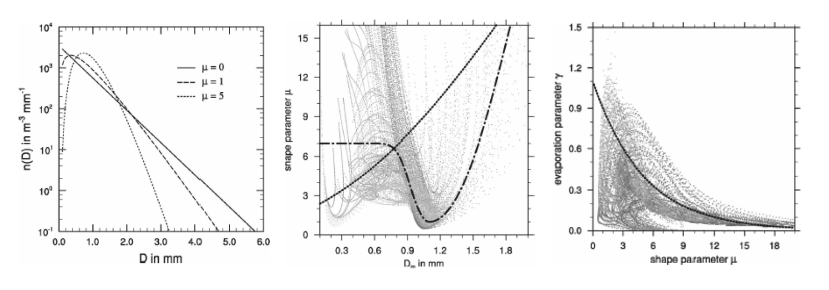
\includegraphics[scale=0.75]{./figure/mod_gamma_dist.eps}
\end{center}
\caption{Left figure shows the modified Gamma distribution for various shape parameters μm. Center figure shows the scatter plot of shape parameter and mean volume diameter for various initial conditions. Gray dots are from the cloud model, dotted line is parameterization of Milbrandt and Yau (2005), and dashed-dotted line is that of Seifert (2008). Right figure shows the scatter plot of evaporation and shape parameters. These are from Seifert (2008).}
\label{figsn2-17}
\end{figure}

\begin{figure}[htbp]
\begin{center}
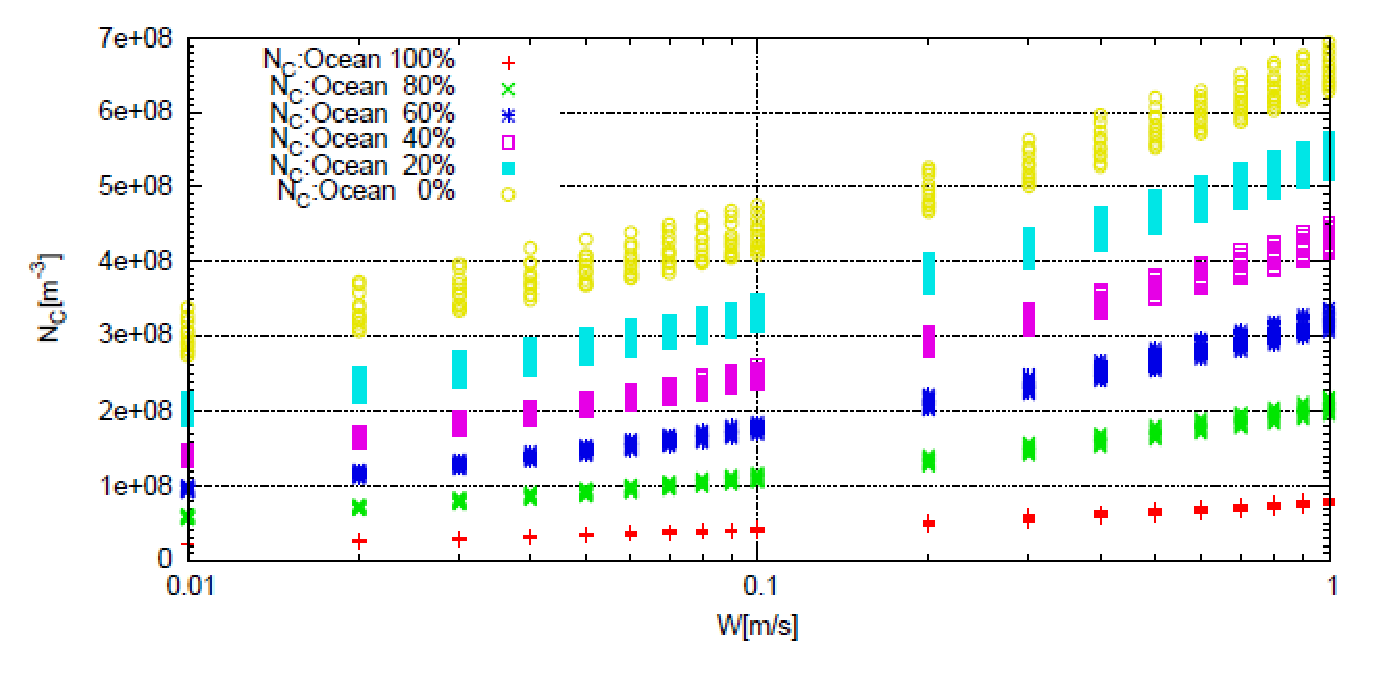
\includegraphics[scale=0.5]{./figure/density_max_num.eps}
\end{center}
\caption{Dependency of maximum number concentration on updraft velocity in ascending air parcel. These are based on a Twomey equation with various CCN conditions. Aerosol activation spectrum refers to eq.\ref{sn107}.}
\label{figsn2-18}
\end{figure}

\begin{figure}[htbp]
\begin{center}
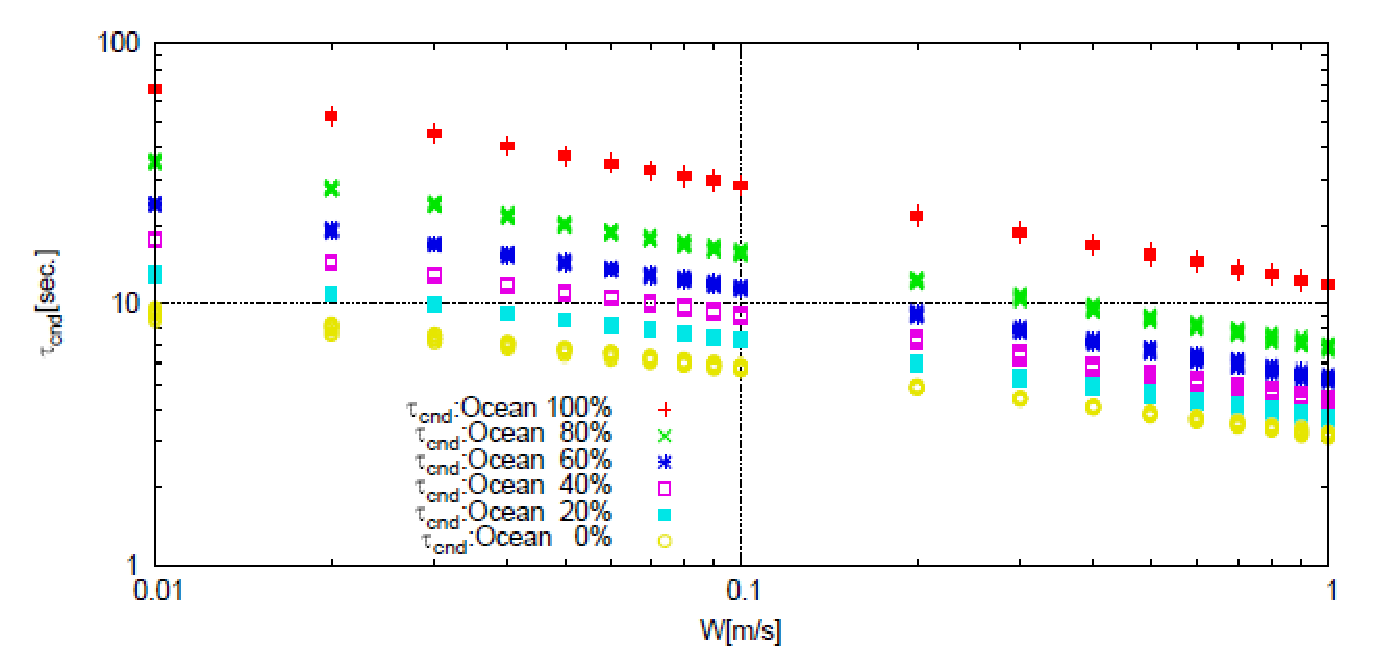
\includegraphics[scale=0.5]{./figure/cond_timescale.eps}
\end{center}
\caption{Timescale of condensation for cloud droplets at maximum number concentration in ascending air parcel. Experimental design is the same as Fig.\ref{figsn2-18}.}
\label{figsn2-19}
\end{figure}

\begin{figure}[htbp]
\begin{center}
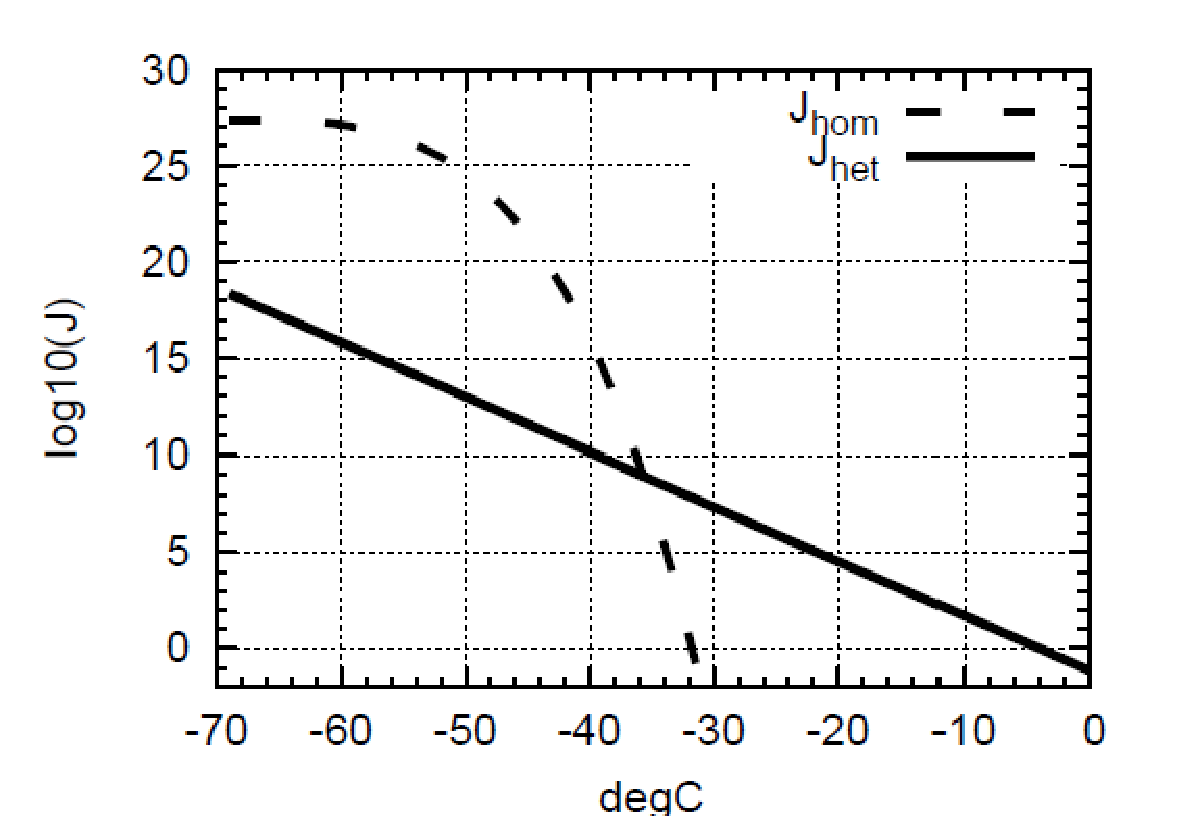
\includegraphics[scale=0.5]{./figure/homo_frz_rate.eps}
\end{center}
\caption{Dependencies of homogeneous freezing rate (dashed line) and heterogeneous freezing rate (solid line) on centigrade temperature. Freezing rates are in common logarithmic scale.}
\label{figsn2-20}
\end{figure}

\begin{figure}[htbp]
\begin{center}
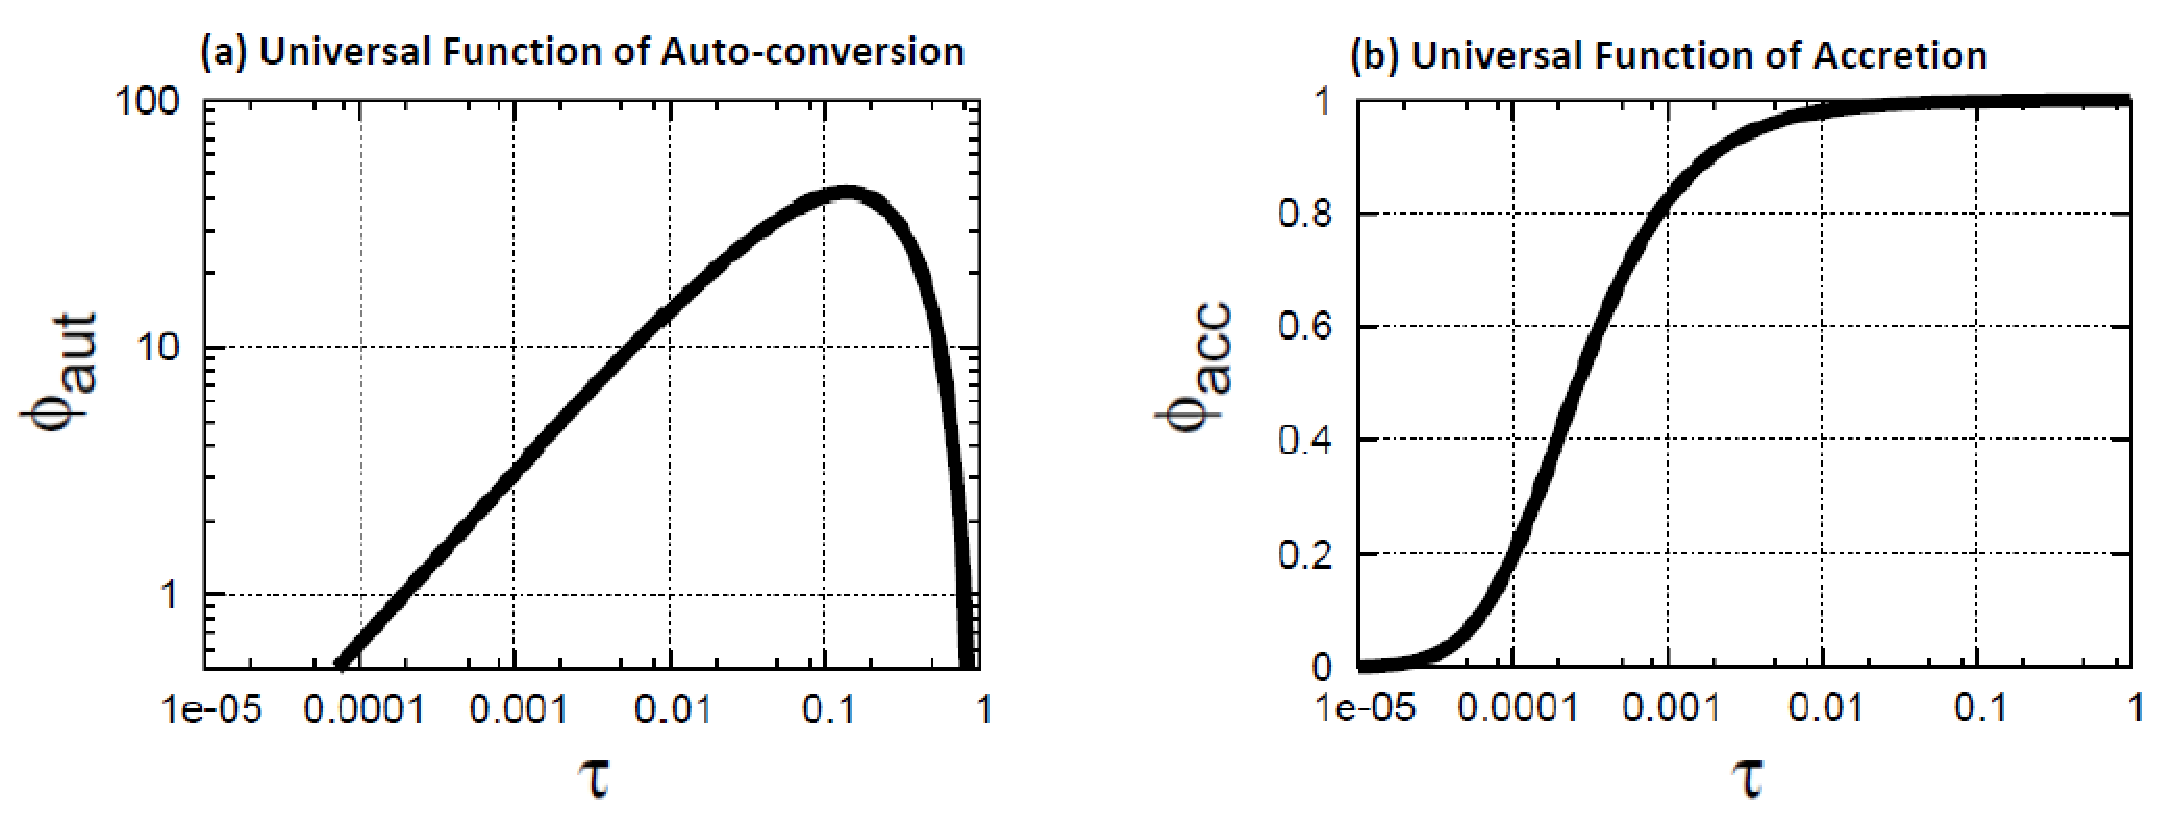
\includegraphics[scale=0.25]{./figure/univ_function.eps}
\end{center}
\caption{The universal functions of (a) auto-conversion and (b) accretion as a function of the dimensionless internal time scale.}
\label{figsn2-21}
\end{figure}

\begin{figure}[htbp]
\begin{center}
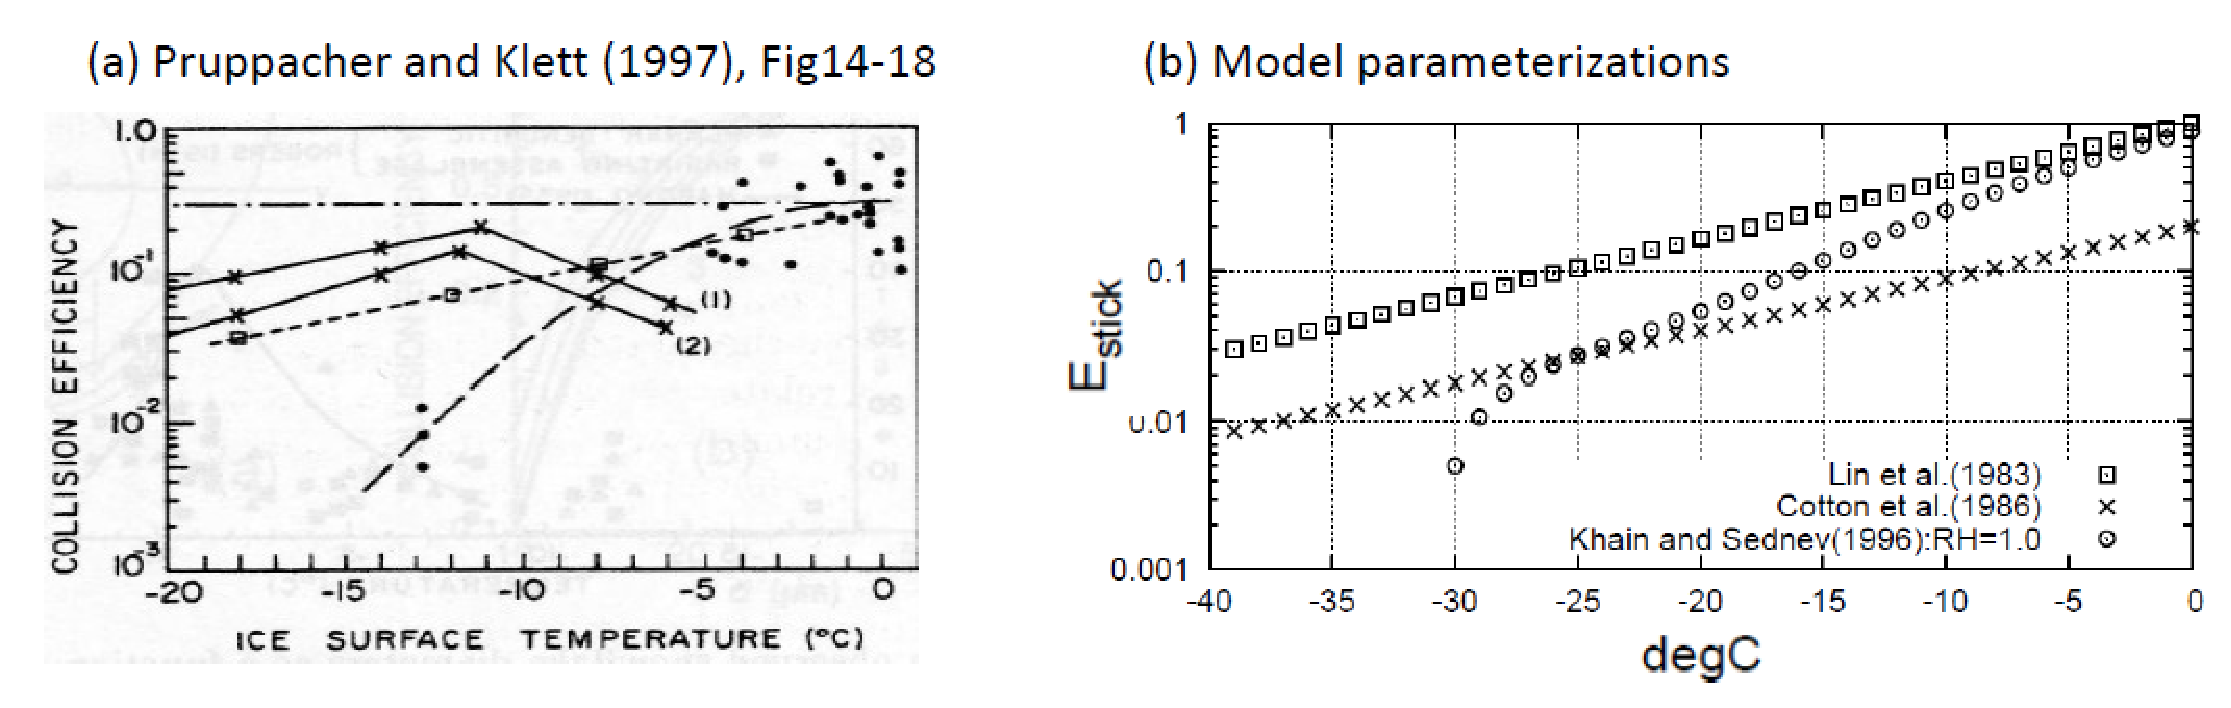
\includegraphics[scale=0.25]{./figure/stic_effic.eps}
\end{center}
\caption{Dependency of sticking efficiencies on centigrade temperature. Sticking efficiencies based on (a) various observations from Pruppacher and Klett (1997) and (b) model parameterizations.}
\label{figsn2-22}
\end{figure}

\begin{figure}[htpb]
\begin{center}
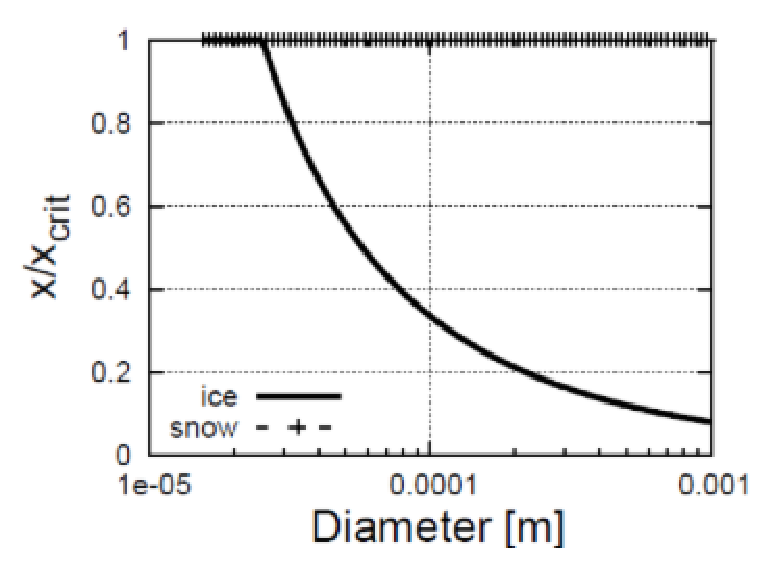
\includegraphics[scale=0.5]{./figure/partial_conversion_coef.eps}
\end{center}
\caption{Coefficients of partial conversion. Solid line shows the coefficient of ice and the line with symbol shows the coefficient of snow.}
\label{figsn2-23}
\end{figure}

\subsubsection{Appendix of Seiki and Nakajima (2014)}
\subsubsection{The k-th moment of generalized Gamma distribution}
The kth moment of the DSD frequently appears in cloud microphysics equations. In this section, we describe derivation of the kth moment of the generalized Gamma distribution. The generalized Gamma distribution is defined as $f(x) = \alpha x \nu exp(-\lambda x \mu)$. There are four parameters in this generalized Gamma distribution but only two prognostic moments in a CRM - the number concentration N and mass concentration L. Hence, $\mu$ and $\nu$ are set constant parameters so that the other coefficients $\alpha$ and $\lambda$ can be related to N and L, as follows:

\begin{eqnarray}
M^{0}=N&=&\alpha\int_{0}^{\infty}x^{\nu}exp(\lambda x^{\mu})dx\nonumber\\
&=&\frac{\alpha}{\lambda^{(\nu+1)/\mu}\mu}\int_{0}^{\infty}y^{(\nu+1)/\mu-1}exp(-y)dy,\;(y\equiv\lambda x^{\mu})\nonumber\\
&=&\frac{\alpha}{\lambda^{(\nu+2)/\mu}\mu}\Gamma\bigl(\frac{\nu+1}{\mu}\bigr)\label{sn255}\\
M^{1}=L&=&\frac{\alpha}{\lambda^{(\nu+2)/\mu}\mu}\Gamma\bigl(\frac{\nu+1}{\mu}\bigr)\nonumber
\end{eqnarray}

$\alpha$ is then expressed as:

\begin{eqnarray}
\alpha=\frac{N\mu\lambda^{(\nu+1)/\mu}}{\Gamma\bigl(\frac{\nu+1}{\mu}\bigr)}=\frac{L\mu \lambda^{(\nu+2)/\mu}}{\Gamma\bigl(\frac{\nu+2}{\mu}\bigr)}\nonumber
\end{eqnarray}

and we can derive $\lambda$ and $\alpha$:

\begin{eqnarray}
\lambda=\Bigl[\frac{\Gamma\bigl(\frac{\nu+1}{\mu}\bigr)}{\Gamma\bigl(\frac{\nu+2}{\mu}\bigr)}\Bigr]^{-\mu}\bar{x}^{-\mu}\;\;and\;\;\alpha=\frac{\nu N}{\Gamma\bigl(\frac{\nu+1}{\mu}\bigr)}\lambda^{(\nu+1)/\mu}\label{sn256}
\end{eqnarray}

where $\bar{x}=L/N$ defines the mean particle mass. We can rewrite the generalized Gamma distribution by using N and L, in the following form:

\begin{eqnarray}
f(x)=\frac{N}{\bar{x}}\bigl(\frac{x}{\bar{x}}\bigr)^{\nu}\frac{\mu}{\Gamma\bigl(\frac{nu+1}{\mu}\bigr)}\Bigl[\frac{\Gamma\bigl(\frac{\nu+2}{\mu}\bigr)}{\Gamma\bigl(\frac{\nu+1}{\mu}\bigr)}\Bigr]^{\nu+1}\exp\Bigl[-\bigl[\frac{\Gamma((\nu+2)/\mu)}{\Gamma((\nu+1)/\mu)}\frac{x}{\bar{x}}\bigr]^{\mu}\Bigr]\label{sn257}
\end{eqnarray}

The kth moment of DSD is now given by the expansion of eq.\ref{sn255} and by using eq.\ref{sn256}:

\begin{eqnarray}
M^{k}=\frac{\Gamma\bigl(\frac{k+\nu+1}{\mu}\bigr)}{\Gamma\bigl(\frac{\nu+1}{\mu}\bigr)}\Bigl[\frac{\Gamma\bigl(\frac{\nu+1}{\mu}\bigr)}{\Gamma\bigl(\frac{\nu+2}{\mu}\bigr)}\Bigr]^{k}N\bar{x}^{k},\;\;(k\in R)
\end{eqnarray}


